\documentclass[11pt]{report}

\usepackage{fancyhdr}
\usepackage{graphicx}
\usepackage{float}
\usepackage{comment}
\usepackage{amsmath}
\usepackage{nicefrac}
\usepackage{commath}
\usepackage{titlesec}
\usepackage{url}
\usepackage[]{algorithm2e}
\usepackage{siunitx}

\renewcommand{\baselinestretch}{1.1}
\pagestyle{fancy} 
\fancyhf{}
%\renewcommand{\chaptermark}[1]{\markboth{\bsc{\chaptername~\thechapter{} :} #1}{\bsc{\chaptername~\thechapter{} :} #1}}
\renewcommand{\sectionmark}[1]{\markright{\thesection{} \ #1}}
\renewcommand{\headrulewidth}{1pt}
\lhead[]{\textsl{\rightmark}}
\rhead[\textsl{\leftmark}]{}
\cfoot[\thepage]{\thepage}

\begin{document}

\RestyleAlgo{boxed}
\LinesNumbered
\begin{titlepage}
	
	\begin{center}
	   
	\vspace*{3cm}
	
	{\Large Individual project Meng 2015}\\[1cm]
	{ \huge \bfseries \textsc{SEMI-RIGID STEREO}}\\[0.2cm]
	
     \vfill
	  	Fran\c{c}ois Berder\\
      Department of Computing\\
      Imperial College London\\

	\end{center}
\end{titlepage}

\chapter*{Abstract}

Stereo vision consists in using multiple images to infer the depth of a scene. Usually, cameras are rigidly fixed such that no relative movement occurs between both cameras. The novelty of this project lies into the semi-rigid aspect: we allow some movement between the left and right camera. First of all, we take a look at various algorithms that may be used later or are similar to the ones actually used. Then, we go through each stage of the semi-rigid stereo processing pipeline which transforms a pair of images into a depth map. In the end, we analyse results.

\chapter*{Acknowledgements}

I would like to thank my supervisor, Stefan Leutenegger, for his support during the entire duration of this project. 

\tableofcontents

\chapter*{Introduction}
\label{chap:Introduction}
\addcontentsline{toc}{chapter}{Introduction}
In recent years, drones became cheaper, more reliable and easier to control generating a wide interest in these small machines. Adding stereo capability would allow them to extend their capabilities such as reconstructing 3D scenes, build maps... However, current stereo solutions are not suited for these drones: a rigid stereo rig would need too much weight and space. Furthermore, stereo works well only if the rig is stable. This characteristic is impossible to maintain due to inevitable vibrations during the flight. In this project, we aim at providing a functional stereo setup made of affordable components that may be be integrated on a small device.

\section{Available Hardware}

I have a pair of Unibrain Fire-I cameras\footnote{Complete specifications available at: http://www.unibrain.com/products/fire-i-digital-camera/\#detailsTab} provided by my supervisor. 


\begin{figure}[H]
  \centering
  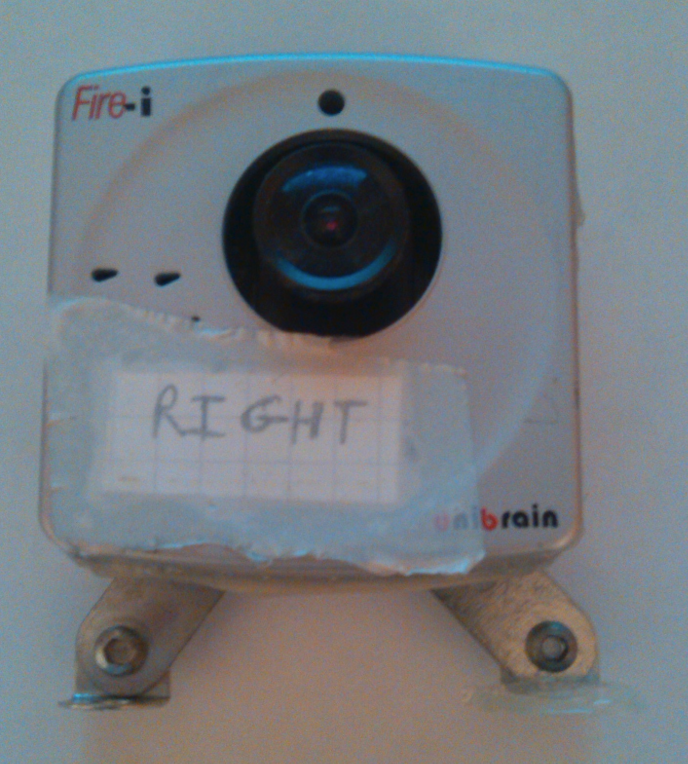
\includegraphics[scale=0.25]{images/camera1.png}
  \caption{Unibrain Fire-i camera}
\end{figure}

\begin{figure}[H]
\centering
\begin{tabular}{|c|c|}
\hline
Interface & Fire-Wire, 2 ports (6 pin) \\
\hline
Speed & 400Mbps \\
\hline
Sensor type & \nicefrac{1}{4}$^{\prime\prime}$ CCD\\
\hline
Pixel shape & Square 5.6$\times$\SI{5.6}{\micro\meter} \\ 
\hline
Focal length & \SI{4.3}{\milli\meter} \\
\hline
Resolutions & $640\times480$, $320\times240$, $160\times120$ \\
\hline
Horizontal view angle & \ang{42} \\
\hline
Vertical view angle & \ang{32} \\
\hline
\end{tabular}
\caption{Camera specifications}
\end{figure}

Parameters can be set using Coriander, a software tool for configuring cameras, such as exposure time, gain, gamma... I also have a 10 meters long Fire-Wire cable and two smaller ones (less than 50 centimetres long) to connect everything. I have a Fire-Wire switch, also provided by my tutor. This switch is very useful because I can use the two small cables to connect the cameras to the switch, and the switch is connected to a computer using the long cable. Hence, I can set the cameras far away from the computer. This is important for outdoors scene because I used a desktop computer with a PCI Fire-Wire card inside.
\begin{figure}[h]
    \begin{center}
        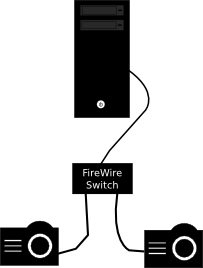
\includegraphics[scale=0.2]{images/setup.png} 
        \label{fig:hardware-schema}
        \caption{Hardware schema}
    \end{center}
\end{figure}

I built a small structure using Mecchano and a flexible plate such that the left camera is still, 12 centimers above the ground, while the right camera can move up and down 5 to 12 centimers above the ground. I can precisely lock the plate at several positions and I can move the plate up and down. To attach the left camera to the plate, I fixed an old part of Mecchano on the plate using a technique called brazing with silver alloy. It appeared that I could not solder newest Mecchano parts on the plate probably because of a change in the composition of the parts which is not compatible with my alloy. Instead, I used a glue gun but it was not effective as the previous solution. I had to re-glue some parts several times. Fortunately, the plate was still flexible after making these changes.

\begin{figure}[H]
  \centering
  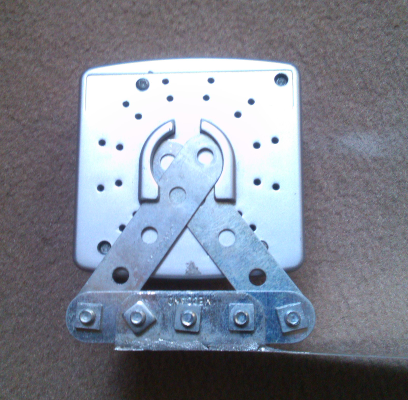
\includegraphics[scale=0.3]{images/attachleft.png}

  \label{fig:attach-left}
  \caption{Back of left camera attached to the plate.}
\end{figure}

\begin{figure}[H]
  \centering
  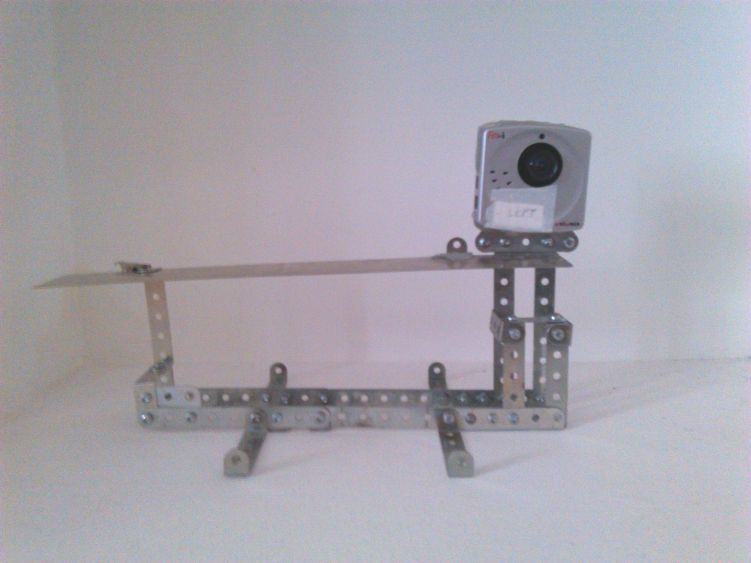
\includegraphics[scale=0.3]{images/rig1.png}
  \label{fig:rig}
  \caption{Stereo rig}
\end{figure}

When both cameras are attached to the plate, the plate bends in the range 2--20 degrees.

\chapter{Background}
\section{Theory}

In this section, we look at the basic math from which stereo is based upon. Most of definitions and results are taken from the book \textit{Multiple View Geometry in Computer Vision, Chapter 9} \cite{Geom}.
 
The general finite projective camera is defined as:
\[
K = 
\left (
\begin{matrix}
	\alpha_x & s & p_x \\
	0 & \alpha_y & p_y \\
	0 & 0 & 1
\end{matrix}
\right )
\]

where $(p_x, p_y)^\top$ is the center of the image and $\alpha_x$ and $\alpha_y$ are the focal length for the horizontal and vertical axis respectively.  In our case, the skew $s$ is zero and $\alpha_x = \alpha_y$. Hence, the matrix can be rewritten as: 
\begin{equation}
K = 
\left (
\begin{matrix}
	f & 0 & p_x \\
	0 & f & p_y \\
	0 & 0 & 1
\end{matrix}
\right )
  \label{eq:camera_matrix}
\end{equation}

$K$ is the camera calibration matrix. It is used to convert points into normalised images coordinates via the equation $\hat{\mathbf{x}} = K\mathbf{x}$.
A pair of projection camera matrices $P$ and $P'$ defines a stereo rig. For convenience, we will always assume that the left camera is at the origin, so $P = [I|0]$. $P'=[R|t]$. Where $t$ is the translation vector from the left camera to the right camera and $R$ is a rotation matrix.

To project point $\mathbf{x} = (X, Y, Z, 1)^\top$ in the left image:
\[
P\mathbf{x} = K[I|0]\mathbf{x} =  K
\left (
\begin{matrix}
	f & 0 & p_x & 0\\
	0 & f & p_y & 0\\
	0 & 0 & 1   & 0
\end{matrix}
\right )
\left (
\begin{matrix}
	X \\
	Y \\
	Z \\
	1
\end{matrix}
\right )
= K
\left (
\begin{matrix}
	fX + Zp_x \\
	fY + Zp_y \\
	Z
\end{matrix}
\right )
\]

The fundamental matrix $F$ describes how a pair of points correspondence $\mathbf{x}' \leftrightarrow \mathbf{x}$ is related: $\mathbf{x}'F\mathbf{x} = 0$. Using the fundamental matrix it is also possible to compute epipolar lines:
\[
  \begin{array}{lcl}
        \mathbf{l}' & = & F\mathbf{x} \\
        \mathbf{l} & = & F^\top\mathbf{x}' \\
  \end{array}
\]

The epipole is the point where all epipolar lines meets, $\mathbf{e}$ and $\mathbf{e}'$ are respectively the left and the right null-vector of $F$. Hence, it verifies the equation $F\mathbf{e} = \mathbf{0}$ and $F^\top\mathbf{e}' = \mathbf{0}$. To compute the epipoles, we use the following formulas:
\[
  \begin{array}{lcl}
        \mathbf{e} & = & KR^\top \mathbf{t} \\
        \mathbf{e}' & = & K'\mathbf{t} \\
  \end{array}
\]

Assuming that $P=[I|0]$, the right epipole is useful to compute a generalised version of $P'$ (this avoids converting points in normalised images coordinates):

\begin{equation}
    P' = [[\mathbf{e}']_xF|\mathbf{e}']
\end{equation}

The essential matrix is a less generalised version of the fundamental matrix. Given a point correspondence in normalised image coordinates $\hat{\mathbf{x}}' \leftrightarrow \hat{\mathbf{x}}$, the essential matrix verifies the equation $\hat{\mathbf{x}}'^\top E\hat{\mathbf{x}} = 0$. And since we know that: $\hat{\mathbf{x}} = K\mathbf{x}$, then $\hat{\mathbf{x}}'^\top E\hat{\mathbf{x}} = \mathbf{x}'K'^\top EK\mathbf{x} = 0$. Hence:

\begin{equation}
	E = K'^\top FK
  \label{eq:essential_matrix}
\end{equation}

Furthermore, in the case of a pair of normalised camera matrices defined as $P =[I|0]$ and $P'=[R|t]$, the essential matrix is :

\begin{equation}
    E = [t]_x R
  \label{eq:essential_matrix2}
\end{equation}

From \ref{eq:essential_matrix} and \ref{eq:essential_matrix2}, we can retrieve $F$:

\begin{equation}
  F = K'^{-\top} [t]_x R K^{-1}
\label{eq:fundamental_matrix}
\end{equation}

From the essential matrix, the rotation matrix $R$ and the translation vector $t$ can then be derived. Let assume that the SVD of $E$ is $Udiag(1, 1, 0)V^\top$, then is possible to factorise $E = SR$, with:
\[
\left .
  \begin{array}{ccl}
        W & = & \left (
                \begin{matrix}
	                0 & -1 & 0 \\
	                1 & 0 & 0 \\
	                0 & 0 & 1 \\
                \end{matrix}
                \right ) \\
        Z & = & \left (
                \begin{matrix}
	                0 & 1 & 0\\
	                -1 & 0 & 0\\
	                0 & 0 & 0 \\
                \end{matrix}
                \right ) \\
        S & = & UZU^\top \\
        R & = & UWV^\top \quad or\quad UW^\top V^\top \\
  \end{array}
\right.
\]
Notice that $W = W^\top$ and $ZW = ZW^\top = diag(1, 1, 0)$. This is used to prove that $E$ can be factorized into $SR$: 
\[
    SR = (UZU^\top)(UWV^\top) = UZWV^\top = Udiag(1, 1, 0)V^\top = E
\]

Using the fact that $E =[t]_x R$ and $E = SR$, so $S=[t]_x$. In addition, $St = \mathbf{0}$ so $t = U(0, 0, 1)^\top$. In other words, $t$ is equal to the last column of $U$. If we assume that left camera matrix $P = [I|0]$, then there are four possible solutions for $P'$:

\[
    [R|t] = K'[UWV^\top | +\mathbf{u}_3] or K'[UW^\top V^\top | +\mathbf{u}_3] or K'[UWV^\top | -\mathbf{u}_3] or  K'[UW^\top V^\top | -\mathbf{u}_3]
\]

To find the correct solution, it is necessary to triangulate a few points and check if most of them are in front of both cameras. In theory, using one point is enough but it may happen that the triangulation fails because of outliers.

\subsection{Triangulation}

I present three triangulation algorithms which I implemented for this project. Further explanations about these algorithms and others are described in \cite{tri97}. The optimal triangulation was implemented from the description in the book \textit{Multiple View Geometry in computer vision (Chapter 12)} by Richard Hartley and Andrew Zisserman\cite{Geom}.

\subsubsection{Linear Eigen triangulation}

This is the simplest triangulation algorithm. Given a 3D point $\mathbf{X}$, it follows that $\mathbf{x} = P\mathbf{X}$ and $\mathbf{x}'=P'\mathbf{X}$. Furthermore, we know that $\mathbf{x} \times (P\mathbf{X}) = \mathbf{0}$. This gives a set of three equations (provided that $\textbf{x}$ is converted into homogeneous form):
\[
\left.
  \begin{array}{rcr}
    x(\mathbf{p}^{3\top}\mathbf{X}) - (\mathbf{p}^{1\top}\mathbf{X}) & = & 0\\
    y(\mathbf{p}^{3\top}\mathbf{X}) - (\mathbf{p}^{2\top}\mathbf{X}) & = & 0\\
    x(\mathbf{p}^{2\top}\mathbf{X}) - y(\mathbf{p}^{1\top}\mathbf{X}) & = & 0\\
  \end{array}
\right.
\]
The last equation is linearly dependent to the first two equations, so we don't use it. Similarly, $\mathbf{x}' \times (P'\mathbf{X}) = \mathbf{0}$ gives two additional equations. The set of four equations are combined in the matrix $A$:

\[
A = 
\left [
  \begin{array}{r}
    x(\mathbf{p}^{3\top}\mathbf{X}) - (\mathbf{p}^{1\top}\mathbf{X}) \\
    y(\mathbf{p}^{3\top}\mathbf{X}) - (\mathbf{p}^{2\top}\mathbf{X}) \\
    x'(\mathbf{p}'^{3\top}\mathbf{X}) - (\mathbf{p}'^{1\top}\mathbf{X}) \\
    y'(\mathbf{p}'^{3\top}\mathbf{X}) - (\mathbf{p}'^{2\top}\mathbf{X}) \\
  \end{array}
\right ]
\]

Hence, we need to solve $A\mathbf{X} = \mathbf{0}$. This is done using a single value decomposition of the matrix $A$ and setting $\mathbf{X}$ as the right eigen vector corresponding to the null eigen value.
However, this method is quite imprecise because it is rarely the case that $\mathbf{x} \times (P\mathbf{X})$ is equal to zero. 

\subsubsection{Mid-point triangulation \cite{Hartley96triangulation}} 

The 3D point is the mid-point belonging to the common perpendicular to the two rays coming from each point. Let assume that the left camera matrix is at the origin and that the translation vector $T$ from the left camera to the right camera is known. Hence, the right camera matrix is at position $t$. Furthermore, the decomposition of the left camera matrix is $\mathbf{P} = [I|\mathbf{0}]$ and the right camera matrix is $\mathbf{P}' = [M' | -M'T]$. Let $\mathbf{l}(\alpha) = \alpha\mathbf{x}$ be the parametric equation of the ray coming from the left image and $\mathbf{l}'(\alpha') = T + \alpha' M'^{-1}\mathbf{x}'$, the parametric equation of the ray coming from the right image (we assume that $\mathbf{x}$ and $\mathbf{x}'$ are in homogeneous coordinates). Since the two rays must intersect, we need to find $\alpha$ and $\alpha'$ such that $\mathbf{l}(\alpha) = \mathbf{l}'(\alpha')$, which gives a set of three equations. Using linear square method, we can find $\alpha$ and $\alpha'$ and compute $\mathbf{X} = \frac{1}{2} (\alpha \mathbf{x} + T + \alpha' M'^{-1} \mathbf{x}')$.

\subsubsection{Optimal solution}

Given a measured point correspondence $\mathbf{x} \leftrightarrow \mathbf{x}'$, the optimal solution computes the points $\hat{\mathbf{x}} \leftrightarrow \hat{\mathbf{x}}'$ that minimises the geometric error and verifies $\hat{\mathbf{x}}'^{\top}F\hat{\mathbf{x}} = 0$. The geometric error is the sum of the squared distance between a point and the corresponding epipolar line:

\[
 \epsilon_{geometric} = d(\mathbf{x}, F\mathbf{x}')^2 + d(\mathbf{x}', F\mathbf{x})^2
\]

To simplify formulas, we assume that $\mathbf{x} = \mathbf{x}' = (0, 0, 1)^\top$ and that the two epipoles are at position $(1, 0 f)^\top$ and $(1, 0, f')^\top$. In this case, the fundamental matrix $F$ has form:

\[
F =
\left (
\begin{matrix}
	ff'd & -f'c & -f'd \\
	-fb & a & b \\
	-fd & c & d
\end{matrix}
\right )
\]

Let assume that the epipolar line in the left image goes through the point $(0, t, 1)^\top$. Then, it also goes through the epipole $(1, 0 f)^\top$. Hence, the vector representing the line is:  $\mathbf{l}(t) = (0, t, 1) \times (1, 0 f) = (tf, 1, -t)$. This is a parametric representation of the epipolar line. The squared distance from the line to the origin ($\mathbf{x}$ is at the origin) is:

\[
    d(\mathbf{x}, \mathbf{l}(t))^2 = \frac{t^2}{1+(tf)^2}
\]

Similarly, the epipolar line in the right image is:
\[
    \mathbf{l}'(t) = F(0, t, 1)^\top = (-f'(ct+d), at+b, ct+d)^\top
\]
The squared distance to $\mathbf{l}'(t)$ is:

\[
    d(\mathbf{x}', \mathbf{l}'(t))^2 = \frac{(ct+d)^2}{(at+b)^2+f'^2(ct+d)^2}
\]

Hence, the total squared distance to minimise is:
\[
    s(t) = \frac{t^2}{1+f^2t^2} + \frac{(ct+d)^2}{(at+b)^2+f'^2(ct+d)^2}
\]

The minimisation translates to finding the roots of the derivate of the function $s$: 
\[
    s'(t) = t((at+b)^2 + f'^2(ct+d)^2)^2 - (ad-bc)(1+f^2t^2)^2(at+b)(ct+d)
\]
This is done using linear gradient descent algorithm. Once the global minimum of $s$ is known at $t_{min}$, we can now compute $\mathbf{l}$ and $\mathbf{l}'$ and find the corrected correspondences $\hat{\mathbf{x}}$ and $\hat{\mathbf{x}}'$:

\[
\left .
  \begin{array}{ccl}
    \hat{\mathbf{x}} & = & (t_{min}^2f, t_{min}, t_{min}^2f^2+1)^\top \\
    \hat{\mathbf{x}}' & = & (f'(ct_{min}+d)(at_{min}+b), -(at_{min}+b)(ct+d), f'^2(ct_{min}+d)^2+(at_{min}+b)^2)\\
  \end{array}
\right .
\]

Finally, the 3D point $\mathbf{X}$ is found using Linear Eigen triangulation with $\hat{\mathbf{x}}$ and $\hat{\mathbf{x}}'$ as input. 

\section{Computing the fundamental matrix}

\subsection{Eight-point algorithm \cite{Geom}}

This is the simplest method for estimating the fundamental matrix $F$ from at least 8 points correspondence. Assuming that a point correspondence $\mathbf{x} \leftrightarrow \mathbf{x}'$ with $\mathbf{x} = (x, y 1)^\top$ and $\mathbf{x}' = (x', y' 1)^\top$, then $F$ verifies $\mathbf{x}'^\top F\mathbf{x} = 0$:

\[
    x'x\mathit{f}_{11} + x'y\mathit{f}_{11} + x'\mathit{f}_{13} + y'x\mathit{f}_{21} + y'y\mathit{f}_{22} + y'\mathit{f}_{23} + x\mathit{f}_{31} + y\mathit{f}_{32} + \mathit{f}_{33} = 0
\]

Let $\mathbf{f}$ a vector made up of the entries of $F$ in row-major order. The equation becomes:

\[
(x'x, x'y, x', y'x, y'y, y', x, y, 1)\mathbf{f} = 0
\]

For $n$ points correspondence, we obtain a set of linear equations of the form:

\[
    A\mathbf{f} = 
\left [
  \begin{array}{ccccccccc}
    x'_1x_1 & x'_1y_1 & x'_1 & y'_1x_1 & y'_1y_1 & y'_1 & x_1 & y_1 & 1 \\
    \vdots & \vdots & \vdots & \vdots & \vdots & \vdots & \vdots & \vdots & \vdots \\
    x'_nx_n & x'_ny_n & x'_n & y'_nx_n & y'_ny_n & y'_n & x_n & y_n & 1 \\
  \end{array}
\right ] 
\mathbf{f} = 0
\]

Using a SVD decomposition of $A$ such that $A = UDV^\top$, the solution vector $\mathbf{f}$ is the last column of $V$.
Due to the fact that $\mathbf{x}'^\top F\mathbf{x}$ is in general not equal to zero because of noise in images, the fundamental matrix $F$ is not singular. To find a singular matrix $F'$ which minimises the frobenius norm $F - F'$ , we use an SVD decomposition of $F$ such that $F = Udiag(r, s, t)V^\top$ with $r \geq s \geq t$ and compute $F' = Udiag(r, s, 0)V^\top$. $F'$ is the output of the eight point algorithm.

The eight-point algorithm must be implemented with care, otherwise it might be too sensitive to noise. Hartley suggested to normalise data\cite{DefenceEightPoint} to reduce errors when enforcing singularity constraint on $F$. Data normalisation consists in computing a transformation $T$ (a translation and a scaling) from a set of points (belonging to the same image) such that the centroid is the origin and the average distance to the origin is $\sqrt{2}$. Let assume that $T$ and $T'$ are transformations for left points and right points set respectively, the algorithm described above finds a solution $\widetilde{F}$ from the normalised data. The denormalized output $F$ is $F = T'^{-1}\widetilde{F}T$. The normalisation ensures that entries of the matrix $A$ have the same order of magnitude which helps reducing errors when $F'$ is replaced by a singular matrix $F$.
The seven-point algorithm is similar to the eight-point algorithm except that it uses the fact that the fundamental matrix has a null determinant.

\subsection{Five-point algorithm}

The five-point algorithm proposed by Nister\cite{FivePointNister04} is able to compute a fundamental matrix from only five points correspondence. Similarly to the eight-point algorithm, it uses the following relationship between points correspondence and the fundamental matrix:

\begin{equation}
  \label{eq:fivepoint1}
  \mathbf{x}'^\top F \mathbf{x} = 0
\end{equation}

However, five points correspondence is not enough to compute the fundamental matrix. In addition, it exploits special properties about the fundamental and essential matrix
\begin{equation}
  \label{eq:fivepoint2}
  \text{det}(F) = 0
\end{equation}

and, 

\begin{equation}
  \label{eq:fivepoint3}
  EE^\top E - \frac{1}{2} trace(EE^\top)E = 0 
\end{equation}

Each constraint from \ref{eq:fivepoint1} can be rewritten as: 

\begin{equation}
  \label{eq:fivepoint4}
  \tilde{q}^\top \widetilde{E} = 0
\end{equation}

with 

\begin{align}
\tilde{q} \equiv \left [ \begin{matrix} \mathbf{q}_1\mathbf{q}'_1 &
  \mathbf{q}_2\mathbf{q}'_1 &
 \mathbf{q}_3\mathbf{q}'_1 &
 \mathbf{q}_1\mathbf{q}'_2 &
 \mathbf{q}_2\mathbf{q}'_2 &
 \mathbf{q}_3\mathbf{q}'_2 &
 \mathbf{q}_1\mathbf{q}'_3 & 
 \mathbf{q}_2\mathbf{q}'_3 &
 \mathbf{q}_3\mathbf{q}'_3
 \end{matrix} \right]^\top \\
\tilde{E} \equiv \left [ 
\begin{matrix}
E_{11} & 
E_{12} & 
E_{13} & 
E_{21} & 
E_{22} & 
E_{23} & 
E_{31} & 
E_{32} &
E_{33} 
\end{matrix}
\right ] ^\top
\end{align}


Constraints obtained from \ref{eq:fivepoint4} are stacked in a $5\times 9$ matrix. After computation of eigen values and their corresponding eigen vectors $X, Y, Z, W$. We can rewrite the essential matrix into a linear combination of the eigen vectors:

\begin{equation}
  \label{eq:fivepoint5}
  E = xX + yY + zZ + wW  
\end{equation}

In the case where more than five points correspondence are used (over-determined case), the four eigen vectors corresponding to the four smallest eigen values are used. Since, $x, y, z, w$ are only defined up to scale, we choose $w=1$. The next step consists in finding the values of $x$, $y$ and $z$. Using result from \ref{eq:fivepoint5} and replacing it into equations \ref{eq:fivepoint2} and \ref{eq:fivepoint3} leads to matrix A (reproduced from \cite{FivePointNister04}):

\begin{center}
\begin{tabular}{|c| c c c c c c c c c c c c c|}
  \hline
  A & $x^3$ & $y^3$ & $x^2y$ & $xy^2$ & $x^2z$ & $x^2$ & $y^2z$ & $y^2$ & $xyz$ & $xy$ & $x$ & $y$ & $1$ \\
  $\langle$a$\rangle$ & 1 & . & . & . & . & . & . & . & . & . & [2] & [2] & [3] \\
  $\langle$b$\rangle$ & & 1 & . & . & . & . & . & . & . & . & [2] & [2] & [3] \\
  $\langle$c$\rangle$ & & & 1 & . & . & . & . & . & . & . & [2] & [2] & [3] \\
  $\langle$d$\rangle$ & & & & 1 & . & . & . & . & . & . & [2] & [2] & [3] \\
  $\langle$e$\rangle$ & & & & & 1 & . & . & . & . & . & [2] & [2] & [3] \\
  $\langle$f$\rangle$ & & & & & & 1 & . & . & . & . & [2] & [2] & [3] \\
  $\langle$g$\rangle$ & & & & & & & 1 & . & . & . & [2] & [2] & [3] \\
  $\langle$h$\rangle$ & & & & & & & & 1 & . & . & [2] & [2] & [3] \\
  $\langle$i$\rangle$ & & & & & & & & & 1 & . & [2] & [2] & [3] \\
  $\langle$j$\rangle$ & & & & & & & & & & 1 & [2] & [2] & [3] \\
  \hline
\end{tabular}
\end{center}
$[N]$ denotes a $N$ degree polynomial in $z$. In addition, we define the following equations: 

\[
  \begin{array}{r c l}
    \langle k \rangle \equiv \langle e \rangle - z \langle f \rangle \\
    \langle l \rangle \equiv \langle g \rangle - z \langle h \rangle \\
    \langle m \rangle \equiv \langle i \rangle - z \langle j \rangle \\
  \end{array}
\]

We can now build a $3\times 3$ matrix $B$ (reproduced from \cite{FivePointNister04}):

\begin{center}
\begin{tabular}{|c| c c c|}
  \hline
  B & x & y & 1 \\
  \hline
  $\langle$k$\rangle$ & [3] & [3] & [4] \\
  $\langle$l$\rangle$ & [3] & [3] & [4] \\
  $\langle$m$\rangle$ & [3] & [3] & [4] \\
  \hline
\end{tabular}
\end{center}

The vector $(x, y, 1)^\top$ is a null-vector to B, so it means that $det(B) = 0$. Hence, we need to solve polynomial $\langle n\rangle$ defined as:

\begin{equation}
  \langle n \rangle \equiv det(B)
\end{equation}

From each root $z$ of $\langle n\rangle$, $x$ and $y$ can be recovered using matrix $B$ and thus the essential matrix E. Since $\langle n \rangle$ is a tenth degree polynomial, there are 10 possible essential matrices but only the one that yields the least error is kept. Finally, the fundamental matrix can be derived from the essential matrix.


\subsection{RAN SAC}

RANSAC\cite{Ransac81} was introduced by Martin A. Fischler and Robert C. Bolles as a new paragdim to extract a model from data. The main advantage of this algorithm lies in its robustness to gross errors in data which is achieved by randomly using a subset of the data to compute a model and check it to the entire dataset. This model finding is realised many times and the best model is the one which has the highest support from data. That is why this algorithm is named RANSAC which stands for RAndom SAmple Consensus. 
There exist many variants of RANSAC to compute the fundamental matrix from a list of points correspondence. Here is one possible version of RANSAC.

\subsubsection{Overview}

The first stage of the algorithm is repeated $N$ times. It selects a small sample of the dataset and use an algorithm to compute the fundamental matrix such as the eight-point algorithm. Afterwards, an error function is evaluated for each pair of points. If the error is less than a predefined threshold, the pair of points is considered as an inlier. Otherwise, it is an outliers. Then, it selects the model which has the highest number of inlier. If several solutions are possible, it keeps the fundamental matrix which has the lowest standard deviation of inlier. Finally, the fundamental matrix is improved by using a non-linear algorithm such as the Levenberg-Marquardt algorithm.

\begin{algorithm}[H]
 \KwIn{A list of pairs of points}
 \KwOut{Fundamental matrix F}
 \tcp{Model estimation}
 \For{N times}{
    Select 8 pairs of points at random\;
    Compute fundamental matrix using the 8-point normalised algorithm\;
    Compute the number of inlier\;
  }
  \tcp{Model selection}
  Select fundamental matrix with highest number of inlier\;
  \tcp{Refinement}
  Use all inlier to refine the fundamental matrix using the Levenberg-Marquardt algorithm
 \caption{Overview of RANSAC algorithm for computing fundamental matrix}
\end{algorithm}

\subsubsection{Computation of $N$}

$N$ depends on the estimated proportion of outliers $\epsilon$ and the probability $p$ that $s$ pertinent points are selected. It follows that a pertinent point is selected with probability $1 - \epsilon$, and $s$ pertinent points are selected with probability $(1 - \epsilon)^s$. Thus, $1 - p = (1 - (1 - \epsilon)^s)^N$. Hence:
\[
    N = \frac{log(1 - p)}{log(1 - (1 - \epsilon)^s)}
\]

Usually, we estimate that 5\% of the data are outliers and we take $p=0.99$. $s$ is the size of the sample for computing $F$ at each iteration. Since we are using the eight-point algorithm $s=8$ but it depends on the choice of the algorithm to compute the fundamental matrix. Alternatively, $N$ can be chosen adaptively to speed up the algorithm. Indeed, the computation of $N$ described above depends on an estimation of the proportion of outliers which may not be correct given the inputs provided. Hence, a lower or greater value of $N$ would be better if it would depend on the measured number of inlier instead.

\subsubsection{Algorithm for computing $F$:}

There exists several algorithms for computing a fundamental matrix from a minimal set of points correspondence. The eight-point algorithm is used by default in the OpenCV library implementation of RANSAC but other algorithms such as the fifth-point algorithm by Nister\cite{FivePointNister04} may be more appropriate for dealing with degenerate data.

\subsubsection{Determining inlier}

A pair of points $x_i' \leftrightarrow x_i$ is considered as an inlier if $d(x_i', Fx_i)$ and  $d(x_i, F^\top x_i')$ are both less than a threshold $t$. Other error functions such as the re-projection error or the Sampson approximation error can also be used.

\subsubsection{Error function in non-linear optimisation}

During the refinement of the fundamental matrix, several error functions can be chosen. I am presenting the cost function described in the version of RANSAC described by A. Zisserman\cite{Ransac97} which is a mix of algebraic and geometric error. The algebraic error $d_i$ for each point correspondence is the shortest distance from a point $x_i$ to the corresponding epipolar line. The geometric error $e_i$ is the re-projection error: the distance between the measured point and the projected point of the 3D point obtained by triangulating the measured points correspondence. The variance of the algebraic and geometric error is also computed, $\sigma$ and $\sigma_l$ respectively. The total error function is:

\[
    D = \sum_i \frac{d_i^2}{\sigma^2} + \sum_i \frac{e_i^2}{\sigma_l^2}
\]

A more robust version of this error function use the Huber function to take into account outliers which introduces some biases in the computation of the variance. Hence, the error function becomes:

\[
    D = \sum_i \gamma(\frac{d_i}{\sigma}) + \sum_i \gamma(\frac{e_i}{\sigma_l})
\]

where $\gamma$ is defined as:

\[
    \gamma(x) = 
\left \{
  \begin{array}{l l}
        x^2 & x < 1.96 \\
        1.96^2 & x \geq 1.96 \\
  \end{array}
\right.
\] 

The value $1.96$ ensures that an inlier is incorrectly rejected in only 5\% of the time.

\subsection{QDEGSAC}

RANSAC works well if the distribution of points in the scene. For instance, if most points lie on a plane, RANSAC often returns degenerate solutions which are only valid for those points but invalid with regards to the reality. To overcome this issue, QDEGSAC\cite{Qdegsac06} is an algorithm built on top of RANSAC.

\begin{algorithm}[H]
  \KwIn{A list of pairs of points}
  \KwOut{Fundamental matrix F}
  \tcp{Initial run}
  Run RANSAC using all data\;
  \tcp{Model selection}
  \While{$\#{inliers}_k \leq t_{red} * \#{inliers}_0$}{
  Run RANSAC using inlier from step $k-1$\;
  }
  \tcp{Model completion}
  Run RANSAC using all outliers from the initial run and inlier from the last step of model selection\;
 \caption{Overview of QDEGSAC algorithm}
\end{algorithm}

The threshold $t_{red}$ is chosen in the range 50\% - 80\% of the number of inlier from the initial run. In practice, the algorithm is not sensitive to the value of $t_{red}$. The goal of the model selection is to remove points which don't add any information. If costs points correspondence lie on the same plane, RANSAC has a high probability to choose only those points and consider any points correspondence not lying on this plane as outliers. By removing some of these points, the probability becomes higher that RANSAC uses some of these points and others to compute a solution. Selecting points lying in different planes does not lead to degenerate solutions.

\section{Levenberg-Marquardt algorithm}

The Levenberg-Marquardt algorithm is a variation of the Gauss-Newton iteration method to minimise a sum of squared function. Let assume $\mathbf{X}$ is a measurement vector which approximates the true measurement vector $\bar{\mathbf{X}}$ and $\mathbf{X} = \mathbf{f}(\mathbf{P})$ where $\mathbf{P}$ is the corresponding parameter vector. We seek to find a parameter vector $\widehat{\mathbf{P}}$ such that $\mathbf{X} = \mathbf{f}(\widehat{\mathbf{P}}) - \epsilon$ where $\mid\mid\epsilon\mid\mid$ is minimised. Although the function $\mathbf{f}$ might not be linear, we assume that it is locally linear. The algorithm starts with a first estimated solution $\mathbf{P}_0$ and compute successive approximations:
\[
  \mathbf{P}_{i+1} = \mathbf{P}_i + \delta_i
\] 

There are several methods to compute $\delta$. The Gauss-Newton method update equation is: 

\begin{equation}
  \label{eq:gauss-newton-update}
  J^\top J\delta = -J^\top \epsilon
\end{equation}

Compared to the Newton method, the Hessian matrix is approximated by $J^\top J$. Another approach is the linear gradient descent algorithm whose update equation is:

\begin{equation}
  \label{eq:linear-gradient-update}
 \lambda \delta = -J^\top \epsilon
\end{equation}

$\lambda$ is a parameter that determines the size of the step. It can either be fixed but this yields poor results or using line search in the downward gradient descent. The novelty of the Levenberg-Marquardt algorithm is that it combines \ref{eq:gauss-newton-update} and \ref{eq:linear-gradient-update}. It transforms the Gauss-Newton update equation $J^\top J\delta = -J^\top \epsilon$ into the equation:

\begin{equation}
  \label{eq:lm_update}
  (J^\top J + \lambda I)\delta = -J^\top \epsilon
\end{equation}
 This speeds up the convergence because the Gauss-Newton does not work well if the function is in a tight corner ($J^\top J$ close to zero). Using a linear gradient descent approach in these situations guarantees a decrease at every iteration.


\subsection{Application to re-projection error minimisation}

The Levenberg-Marquardt is only used in this project to minimise the re-projection error of a fundamental matrix $F$ given a list of 3D points obtained by triangulation. The measurement vector $\mathbf{X} = (\mathbf{X}_1, \mathbf{X}_2, \hdots, \mathbf{X}_n)^\top$ where each $\mathbf{X}_i = (\mathbf{x}_i^\top, \mathbf{x}'^\top_i)^\top$ contains the $i$-th measured pair of points.
The parameter vector $\mathbf{P}$ is split into $\mathbf{a}$ and $\mathbf{b}$, thus $\mathbf{P}=(\mathbf{a}^\top, \mathbf{b}^\top)^\top$. $\mathbf{a}$ is a 12-vector made up of the entries of the right projection matrix P' (which can be derived from the fundamental matrix $F$) and $\mathbf{b}=(b_1, b_2, \hdots, b_n)^\top$ where $b_i = (X_i, Y_i, T_i)^\ast$ is a 3-vector of the $i$-th 3D point $(X_i, Y_i, 1, T_i)^\top$. The function $\mathbf{f}$ is the projection function: $\mathbf{f}(\mathbf{P}', \mathbf{b}_i) = (P\mathbf{b}_i, P'\mathbf{b}'_i)^\top = (\widehat{\mathbf{x}}_i^\top, \widehat{\mathbf{x}}'^\top_i)^\top = \widehat{\mathbf{X}}_i$.

Due to the structure of the parameter vector $\mathbf{P}$, the Jacobian matrix becomes $J = \left [ \frac{\partial\widehat{\mathbf{X}}}{\partial \mathbf{P}} \right ]$ is made of two blocks $J=\left [ A\mid B\right ]$ where:

\[
A = \left [ \frac{\partial\widehat{\mathbf{X}}}{\partial\mathbf{a}}\right ]
\]
and
\[
B = \left [ \frac{\partial\widehat{\mathbf{X}}}{\partial\mathbf{b}}\right ]
\]

The normal equation \ref{eq:lm_update} becomes: 

\begin{equation}
    \label{eq:lm_update2}
    \left ( 
    \begin{matrix}
        A^\top\Sigma^{-1}_{\mathbf{X}}A &  A^\top\Sigma^{-1}_{\mathbf{X}}B \\
        B^\top\Sigma^{-1}_{\mathbf{X}}A &  B^\top\Sigma^{-1}_{\mathbf{X}}B \\
    \end{matrix}
    \right )
    \left (
    \begin{matrix}
      \delta_A \\
      \delta_B \\
    \end{matrix}
    \right )
    =
    \left (
    \begin{matrix}
        A^\top\Sigma^{-1}_{\mathbf{X}}\epsilon \\
        B^\top\Sigma^{-1}_{\mathbf{X}}\epsilon \\
    \end{matrix}
    \right )
\end{equation}

If the covariance matrix $\Sigma^{-1}_{\mathbf{X}}$ is not known then it can be replaced by the identity matrix. To simplify notations, we introduce matrices U, V and W;

\[
    \left ( 
    \begin{matrix}
        A^\top\Sigma^{-1}_{\mathbf{X}}A &  A^\top\Sigma^{-1}_{\mathbf{X}}B \\
        B^\top\Sigma^{-1}_{\mathbf{X}}A &  B^\top\Sigma^{-1}_{\mathbf{X}}B \\
    \end{matrix}
    \right )
=
\left (
  \begin{matrix}
      U & W \\
      W^\top & V \\
  \end{matrix}
\right )
\]

Equation \ref{eq:lm_update2} is simplified to:

\begin{equation}
  \label{eq:lm_update3}
  \left (
    \begin{matrix}
        U & W \\
        W^\top & V \\
    \end{matrix}
  \right )
  \left (
  \begin{matrix}
    \delta_A \\
    \delta_B \\
  \end{matrix}
  \right )
  = 
  \left (
  \begin{matrix}
    \epsilon_A \\
    \epsilon_B \\
  \end{matrix}
  \right )
\end{equation}

To find $\delta_A$ and $\delta_B$, we multiply each side of the equation \ref{eq:lm_update3} on the left by $\left [ \begin{matrix} I & -WV^{\ast -1} \\ 0 & I \\ \end{matrix} \right ]$:

\begin{equation}
  \label{eq:lm_update4}
  \left (
    \begin{matrix}
        U^\ast - WV^{\ast -1}W^\top & 0 \\
        W^\top & V^\ast \\
    \end{matrix}
  \right )
  \left (
  \begin{matrix}
    \delta_A \\
    \delta_B \\
  \end{matrix}
  \right )
  = 
  \left (
  \begin{matrix}
    \epsilon_A - WV^{\ast -1}\epsilon_B \\
    \epsilon_B \\
  \end{matrix}
  \right )
\end{equation}

From equation \ref{eq:lm_update4}, we obtain the following equations:

\begin{equation}
  (U^\ast - WV^{\ast -1}W^\top)\delta_A = \epsilon_A - WV^{\ast -1}\epsilon_B
\end{equation} 

\begin{equation}
  V^\ast\delta_B = \epsilon_B - W^\top\delta_A
\end{equation} 


Furthermore, the computation of the solution $\delta$ of the normal equation \ref{eq:lm_update} is of complexity $N^3$. We need to take into account the fact that $J$ has a special structure. The Jacobian matrix $J$ is mostly full of zeros because each entry $\mathbf{b}_i$ is independent from each other and is related with only $\mathbf{a}$. Hence, we are using a sparse variant of the Levenberg-Marquardt algorithm.

The computation of each partial derivative matrix $A_i$:

\begin{equation}
A_i = \frac{\partial\widehat{\mathbf{X}}_i}{\partial\mathbf{a}} = \frac{\partial\mathbf{f}(\mathbf{a}, \mathbf{b}_i)}{\partial\mathbf{a}} = 
\left [ 
  \begin{matrix}
    \frac{\partial \widehat{\mathbf{x}}_i}{\partial\mathbf{a}} \\
    \frac{\partial \widehat{\mathbf{x}}'_i}{\partial\mathbf{a}} \\
  \end{matrix}
\right ]
= 
\left [ 
  \begin{matrix}
    0 \\
    \frac{\partial \widehat{\mathbf{x}}'_i}{\partial\mathbf{a}} \\
  \end{matrix}
\right ]
\end{equation}

The computation of each partial derivative matrix $B_i$:
\begin{equation}
B_i = \frac{\partial\widehat{\mathbf{X}}_i}{\partial\mathbf{b}} = \frac{\partial\mathbf{f}(\mathbf{a}, \mathbf{b}_i)}{\partial\mathbf{b}} =
 \left [ 
  \begin{matrix}
    I_{2\times 2} \mid \mathbf{0} \\
    \frac{\partial \widehat{\mathbf{x}}'_i}{\partial\mathbf{b}} \\
  \end{matrix}
\right ]
\end{equation}

\begin{algorithm}[H]
  \KwIn{A list of pairs of points}
  \KwIn{Initial estimation of fundamental matrix $F_{initial}$}
  \KwOut{refined Fundamental matrix F}
  \tcp{Triangulation}
  Triangulate each pair of points to obtain a list of 3D points $\mathbf{X}_i$\;
  \tcp{Iterative minimisation}
  \Repeat{$\abs{error_{k} - error_{k-1}} < t$}{
    \tcp{Compute $A_i$ and $B_i$}
    $A_i = \left [ 0 \right ]$\;
    $B_i$\;

    \tcp{Compute error vector}
    $\epsilon_i = \mathbf{X}_i - \widehat{\mathbf{X}}_i$\;

    \tcp{Compute covariance matrices}
    $\Sigma_{\mathbf{X}_i}$ = diag$(S_i, S_i')$ where $S_i = \Sigma_{\mathbf{x}_i}^{-1}$ and $S_i' = \Sigma_{\mathbf{x}_i'}^{-1}$\;

    \tcp{Compute intermediate results}
    U = $\sum_iA^\top_i\Sigma^{-1}_{\mathbf{X}_i}A_i$\;
    V = diag$(V_1, \hdots, V_n)$ where $V_i = B^\top_i\Sigma^{-1}_{\mathbf{X}_i}B_i$\;
    W = $\left [ W_1, W_2, \hdots, W_n \right]$ where $W_i = A^\top_i\Sigma^{-1}_{\mathbf{X}_i}B_i$\;
    $\epsilon_A = \sum_iA^\top_i\Sigma^{-1}_{\mathbf{X}_i}\epsilon_i$\;
    $\epsilon_B = (\epsilon^\top_{B_1}, \epsilon^\top_{B_2}, \hdots, \epsilon^\top_{B_n})^\top$ where $\epsilon_{B_i} = B^\top_i\Sigma^{-1}_{\mathbf{X}_i}\epsilon_i$\;
    $Y_i = W_iV_i^{\ast-1}$\;
  
    \tcp{Augment U and V}
    $U^\ast = U + \lambda I$\;
    $V^\ast = V + \lambda I$\;

    \tcp{Compute $\delta_A$ and $\delta_{B_i}$}
    $\delta_A = (\epsilon_A - \sum_iY_i\epsilon_{B_i})(U^\ast - \sum_iY_iW_i^\top)^{-1} $\;
    $\delta_{B_i} = V^{\ast-1}(\epsilon_{B_i} - W_i^\top \delta_A)$\; 

    \tcp{Compute new parameter vector}
     $A_{k+1} = A_k + \delta_A$\;
     $B_{i, k+1} = B_{i, k} + \delta_{B_i}$\;

    \tcp{Compute error}
    $error_{k+1}$ = reprojectionError(A, B)\;

    \If{$error_{k+1} < error_k$}{
      Accept new parameters\;
      Diminish $\lambda$ by a factor of 10\;
    }
    \Else{
      Increase $\lambda$ by a factor of 10:
    }
  }
 \caption{Complete description of the sparse Levenberg-Marquardt algorithm for minimising re-projection error \cite{Geom}}
\end{algorithm}

\section{Stereo matching algorithm}

These algorithms compute a disparity map from a pair of images. They also assume that images are rectified: epipolar lines are parallel to the x-axis. This constraint simplifies tremendously the computation of a disparity map since algorithms only have to compare pixels between each line of the  A disparity map is a black and white image where the intensity of each pixel indicates by how much pixels the left and right images differs. This means that objects near the cameras will appear brighter in the disparity map than farther objects. The disparity map must not be be confused with the depth map. Even though the depth map is computed from the disparity map, the later does not hold any information about distances.
Stereo matching algorithms can be divided into two classes: local stereo matching and global stereo matching. Global stereo matching computes more accurate disparity maps than the former but they are considerably slower than local stereo matching algorithms and thus, they are not suitable for real-time applications.

\subsection{Local Stereo matching}

Local stereo matching operates on pixel level and compares then between left and right images. Most of these algorithms respect the left-right consistency constraint: a 3D point can only be projected once in the left and right image. Hence, a pixel from the left image can be associated with at most one pixel from the right image and vice versa. Not all pixels from one image can be associated with a pixel belonging to other pixel due to occlusions, or photometric distortions.
To respect this constraint, most of algorithms use bidirectional matching: they start with associating each pixel from the left image with a pixel from the right image. The same operation is done this time associating pixels from the right image with pixels from the left image. Then, only matches that are coherent while matching from left to right and right to left are kept. Even though this approach handles well occlusions, it requires two matching phases. That is why, we will have a look at a fast stereo local stereo matching presented by L. Di Stefano, M. Marchionni, S. Mattoccia and G. Neri\cite{Stefano02afast}.
This algorithm works in four steps:
\begin{enumerate}
  \item \textbf{Pre-Processing} This step aims at eliminating small distortions caused by the different properties of each camera used to capture images. The value of each pixel is subtracted by the mean value of the intensities computed from a small window center on the pixel. Along the mean intensity, the variance is also computed to provide additional information in stage 3 to handle poorly textured areas.

  \item \textbf{Basic Matching Core}
The main novelty of this algorithm lies in the basic matching core. Instead of using bidirectional matching, it uses another one local algorithm called single matching phase (SMP). Let assume that pixel in left image at position $(x, y)$ is represented by $L(x, y)$. Similarly, $R(x, y)$ is the pixel at position $(x, y)$ in the right image. For $L(x-d_{max}, y)$, the algorithm evaluates an error function $\varepsilon$ on the interval $[R(x-d_{max}, y), \hdots, R(x,y)]$. This step is repeated for each pixel belonging to the same line. It may happen that two pixels $L(x+\alpha - d_{max}, y)$ and $L(x+\beta - d_{max}, y)$ with $\alpha \leq \beta$ are both associated with $R(x, y)$: this is a collision. The collision is avoided by retaining the pixel which has the highest score (least error).

  \item \textbf{Reliable Tests}

The previous stage is more error-prone than bidirectional matching, especially when dealing borders of objects. SMP assumes that the entire interval $[R(x-d_{max}, y), \hdots, R(x,y)]$ may contain a potential match for $L(x, y)$. However, this is wrong if this interval contains depth discontinuities. Hence, only a subset of the interval is valid. To overcome this issue, it uses the position of the three local minimums and the global minimum to compute $\delta d$:

\begin{equation}
  \delta d = \sum_{i=1}^{3} \mid d_i - d_{min} \mid 
\end{equation}

A low value of $\delta d$ means that the potential match is likely to be valid because these three local minimums are close from the global minimum. On the other hand, if $\delta d$ is too high, then it is considered as an ambiguous match. In this case, it performs an additional test: it checks how distinctive is the global minimum compared to the local minimums.

\begin{equation}
  \delta \varepsilon = \sum_{i=1}^{3} (\varepsilon_i - \varepsilon_{min}) 
\end{equation}

If the value $\frac{\delta \varepsilon}{\varepsilon_{min}}$ is high, then it means that the match is nonetheless correct because the global minimum is very distinctive from the rest. Otherwise, it discards the match.

  \item \textbf{Sub-Pixel Measurement}

The last step consists in refining the disparity up to $1/16$ of pixel by finding the minimum of a second degree curve using scores computed in stage 2 around the global minimum.
\end{enumerate}

\section{Feature point detection and matching}
A solution to this project relies on three algorithms. A feature point detector generates a list of feature points from both images. Then, these points. Since the detection and matching of feature points are so dependent on each other, it is common than algorithms handle these two cases together: first, they present a feature point detector, then they describe an algorithm to match these points compared to a database. I considered algorithms which have an implementation in the OpenCV library.

\subsection{Moravec}
Feature point detection started by detecting corners. One the first corner detector was described by Moravec in 1980\cite{Moravec80} such that a seeing robot could move while avoiding obstacles. It works by detecting changes in intensity of a small window shifted in several directions. If there is at least one large changes in one direction, then the center of the window will be kept as a feature point. The shift $E$ around a point at $(x,y)$ can be computed from the following equation:

\begin{equation}  
  \label{eq:moravec}
  E(x,y) = \sum_u \sum_v w(u, v) (I(x+u, y+v) - I(u,v))^2
\end{equation}


$w$ is either equal to the unity in a specified rectangular section and zero elsewhere. This algorithm has several drawbacks. First of all, it considers only a small set of directions. It does not take into account that pixels are rectangular due to the definition of $w$ and reacts too much on edges. Indeed, consider a white line over a black background, using this algorithm most points on the line have huge variations with surrounding points except in two directions. Hence, it will probably consider most points belonging to this line as good candidates for feature points.

\subsection{Harris detector}
Eight years later, Harris and Stephens published a paper\cite{Harris88} about a new feature point detector that detects corners and edges in order to address some weaknesses of the previous algorithm by changing  equation \ref{eq:moravec}. First of all, $w$ is now defined using a Gaussian:

\[
  w(u, v) = e^{-\frac{u^2+v^2}{2\sigma^2}}
\]

This means that a smooth circular window is used instead of a rectangular one.
Then, $I(u+x, v+y)$ is approximate to $I(u+v) + \frac{\partial I}{\partial x} + \frac{\partial I}{\partial y}$. $E(x, y)$ becomes:

\[
E(x, y) \approx \sum_u \sum_v w(u, v) \left ( \frac{\partial I}{\partial x}(u, v)x + \frac{\partial I}{\partial y}(u, v)y \right ) ^2
\]

We can now rewrite $E$ in matrix form:

\[
E(x,y) \approx (x,y) M  \begin{pmatrix}x\\y\end{pmatrix}
\]

where M is defined as:

\[
  M =  \sum_u \sum_v w(u, v) \left [ \begin{matrix} \frac{\partial^2 I}{\partial^2 x} & \frac{\partial I}{\partial x} \frac{\partial I}{\partial y} \\ \frac{\partial I}{\partial x} \frac{\partial I}{\partial y} & \frac{\partial^2 I}{\partial^2 y} \end{matrix} \right ]
\]

The eigenvalues $\alpha$ and $\beta$ of the matrix M are computed. Ideally, an edge is detected is one of these values is zero and the other one is large. Because of noise, pixellation and intensity encoding (probably limited to one byte in monochrome images), it is very unlikely to happen that one eigenvalue is zero, more often one eigenvalue is large and the other one is small. In case of a corner, both eigenvalues are large. If both eigenvalues are small, then this is a flat region. This algorithm depends on a threshold to determine whether eigenvalues are small or large. One drawback of this algorithm is that it is not scale-invariant.


\subsection{Good features to track}
There are other situations where early algorithms failed to detect good feature points. For instance, small reflections on a glossy surface or a corner created by two objects at different depths may be picked as a good feature point using \textit{cornerHarris}. To detect and remove these bad feature points, Jianbo Shi and Carlo Tomasi developed an algorithm\cite{Shi94} which works on a sequence of images. Instead of applying they algorithm to only one image, they apply it to a sequence. First, they apply a feature detector to the first image. This gives a list of candidate feature points. Then, for each of those, it computes the dissimilarity between the first image and the rest of the images in order. If this dissimilarity function does not increase, then the feature point associated with is probably a good feature point (a corner of a real 3d object). Otherwise, it is discarded.

\subsection{FAST detector}

To improve the speed of these feature detectors, the FAST\cite{Fast06} algorithm works in three stages. 

\subsubsection{Segment test detector}
First, it performs a quick test to detect if this candidate is likely to be a corner. Up to sixteen pixels, belonging to a circle whose candidate corner is the center, are used for this test. It uses only pixel 1, 5, 9 and 13. If at least three of them match this criteria: $I < I_p - t$ or $I > I_p + t$, then it checks against the remaining 12 pixels. At this stage, if n pixels (out of 16) follow the previous criteria, another test will be performed for this candidate corner. During the quality testing of this algorithm, best results were found for $n = 9$. This test has several drawbacks, notably it does not eliminate adjacent corners. Hence a final stage is needed to remove them.

\subsubsection{Learned detector}
The second stage was built using machine learning. For each candidate corner found by the first stage, 

\begin{enumerate}
	\item It compares each pixel $x$ belonging to the circle to all other pixels. This creates three sets $S_s$, $S_d$ and $S_b$.
	\item It computes the entropy of each set. $H(P) = (c + \bar{c})\log_2{c + \bar{c}} + c\log_2{c} + \bar{c}\log_2{\bar{c}}$
	\item For each $x$, it selects $x$ which has the most information gain $H(P) - H(P_s) - H(P_d) - H(P_d)$
	\item It repeats this algorithm but using $S_s$, $S_d$ and $S_b$ instead of the set S.
\end{enumerate}

This function is guaranteed to terminate and a decision tree can be induced from it. This decision tree is then transformed into C code and compiled.

\subsubsection{Non-maximal suppression}
In the end, it computes a score for each detected corner to eliminate those adjacent to a better corner.
\[
V = max \left(\sum_{x \in S_{bright}}{\abs{I_{p \rightarrow x} - I_p} - t},  \sum_{x \in S_{dark}}{\abs{I_p - I_{p \rightarrow x}} - t} \right)
\]
with,
\[
	x \in S_{bright} \Leftrightarrow  I_{p \rightarrow x} \geq I_p + t
\]
\[
	x \in S_{bright} \Leftrightarrow  I_{p \rightarrow x} \leq I_p + t
\]

The performance improvement is significant: about thirty times faster on a Pentium III 850MHz over the Harris detector.

\subsection{SURF}

SURF\cite{Surf06} is a feature detector that associate each feature with a descriptor to allow feature matching across different images. The descriptor is scale-invariant as well as rotation invariant. This means that despite having different size or orientations, similar features can be matched.

\subsubsection{Feature point detection}

 For each pixel in the image, a Hessian matrix $H$ is built: 
\[
  H(\mathbf{x}, \sigma) =
  \left [
  \begin{matrix}
    L_{xx}(\mathbf{x}, \sigma) & L_{xy}(\mathbf{x}, \sigma) \\
    L_{xy}(\mathbf{x}, \sigma) & L_{yy}(\mathbf{x}, \sigma)
  \end{matrix}
  \right ]
\]

where $L_{xx}(\mathbf{x}, \sigma)$ is the Gaussian second order derivative, i.e. $\frac{\partial^2 g(\sigma)}{\partial^2 x}$. The derivative is approximate using a box filter $D$ to reduce computation time.  The determinant of the Hessian matrix $H$ is then approximated to:

\[
det(H) \approx D_{xx}D_{yy} - (0.9D_{xy})^2
\]

If $det(H)$ is greater than a threshold, then the point is kept as a feature point.
To achieve scale invariance, the previous step is performed several times not by scaling down the image as in SIFT\cite{Sift04} but instead scaling up the box filter. The size, in pixel, of each box filter are : $9\times9$, $15\times15$, $21\times21$ and $27\times27$.  Also, the parameter needs to be adjusted accordingly to the size of the box filter. $\sigma$ is equal to 1.2 for box filter of size $9\times9$, 3.6 for size $27\times27$, etc. After this step, a threshold is used to keep control on the number of feature detectors. Finally, A non-maximum suppression is applied in a 3x3x3 neighbourhood. The coordinates of this neighbourhood are x, y, and s (the scale factor of the box filter).

\subsubsection{Feature point descriptor}

The SURF descriptor is a simplified variant of the SIFT descriptor. First, the orientation of the feature point is determined. The Haar-Wavelet respond is computed in the $x$ and $y$ directions in a circular neighbourhood of size $6s$. The wavelets are weighted with a Gaussian ($\sigma = 2.5s$) centered on the feature point. Each wavelet is plotted on a graph where the abscissa is the horizontal response and the ordinate is the vertical response. The sum of all responses within a sliding window covering an angle of $\frac{\pi}{3}$ is computed. The sum yields a vector, and the longest vector indicates the dominant orientation of the feature point. 

The feature descriptor is computed from a square region of size $20s$ oriented along the orientation computed previously. This region is split into smaller sub-region of size $4\times4$ and the Haar Wavelet response, $dx$ and $dy$, is computed at  $5\times5$ regularly space point in the horizontal and vertical direction. $dx$ and $dy$ are weighted using a Gaussian ($\sigma=3.3s$) to increase the robustness of the descriptor towards geometric deformation and localisation errors. Each sub-region is described by the vector $v$:

\[
v = (\sum{dx}, \sum{dy}, \sum{\abs{dx}}, \sum{\abs{dy}})
\]

The vector $v$ is normalised to achieve invariance to contrast. The complete SURF descriptor is a set of 16 vectors $v$.

\subsection{ORB}

ORB\cite{Orb11} is a mix of FAST, SIFT and BRIEF to create a more robust and faster feature point detector and descriptor. Let $N$ be the number of feature points to be detected. Using a low enough threshold, more than $N$ feature points are detected using FAST-9 (circular radius of 9 pixels). For each feature point, the Harris corner measure (sum of $\alpha$ and $\beta$) is computed to order the set of feature points. The best $N$ feature points are kept. Like SURF, it employs this technique over a scale pyramid to achieve scale invariance.

The orientation of the feature point is based on the assumption that the feature point $O$ is shifted from the intensity centroid $C$. The moment of a patch is defined as:

\begin{equation}
  \label{orb:moments}
  m_{p,q} = \sum_{x,y} x^py^q I(x,y)
\end{equation}

From \ref{orb:moments}, the centroid $C$ can be computed as :

\[
  C = \left ( \frac{m_{10}}{m_{00}}, \frac{m_{01}}{m_{00}} \right )
\]

Using the four quadrant inverse arctangent, the orientation $\theta$ of the vector $\overrightarrow{OC}$ is:

\[
  \theta = \text{atan2}(m_{01}, m_{10})
\]

ORB feature descriptor is based on the BRIEF feature descriptor \cite{Brief10}. The descriptor is a bit string describing the results of a set of binary intensity tests. Let assume a smooth patch of size $5\times 5$ centered on points $\mathbf{x}$ and $\mathbf{y}$. A binary test $\tau$ is defined as:

\[
  \tau (\mathbf{p}, \mathbf{x}, \mathbf{y}) =   
\left \{
  \begin{array}{l l}
    1 & \mathbf{p}(\mathbf{x}) < \mathbf{p}(\mathbf{y}) \\
    0 & \mathbf{p}(\mathbf{x}) \geq \mathbf{p}(\mathbf{y}) \\
  \end{array}
  \right .
\]

where $\textbf{p}$ is the intensity of the patch. The feature descriptor $f$ is:

\[
  f_n(\mathbf{p}) = \sum_{1 \leq i \leq n}  2^{i-1} \tau(\mathbf{p}, \mathbf{x}, \mathbf{y})
\]

Like BRIEF, ORB has a feature descriptor of length equal to 256 ($n=256$). Hence there are $n$ binary tests comparing a $n$ pair of patches at location $\mathbf{x}_i$ and $\mathbf{y}_i$. This defines a $2\times n$ matrix:

\[
\mathbf{S} = 
\left ( \begin{matrix} 
\mathbf{x}_1 & \hdots & \mathbf{x}_n \\
\mathbf{y}_1 & \hdots & \mathbf{y}_n \\
\end{matrix} \right )
\]

The novelty of ORB lies in transforming the matrix $S$ with the orientation $\theta$ computed earlier. A new matrix $S_\theta$ is defined as:

\[
  S_\theta = R(\theta)S
\]

The feature descriptor becomes:

\[
  g_n(\mathbf{p}, \theta) = f_n(\mathbf{p}) \mid (\mathbf{x}_i, \mathbf{y}_i) \in S_\theta
\]

This feature descriptor has lower variance among bits than BRIEF because BRIEF assumes a random orientation among all feature points. High variance among the feature descriptor is needed because it makes the feature more unique and less mismatch will occur during feature point matching. One simple solution would consist in increasing the size of the feature descriptor but it would have a performance impact on the algorithm. Another solution consists in identifying 256 pairs of locations from a bigger patch that are not correlated. Using a training set of some 300k key-points, all possible binary tests from a $31\times 31$ pixel patch are considered. Each test is a pair of $5\times 5$ subregions of the patch. This means that there are 205590 possible tests for each key-point. After running each test, they are ordered according to their distance to a mean of 0.5 to form a vector $T$. Then, a greedy search is performed on T to build a result vector R.

\begin{algorithm}[H]
  \KwIn{Vector T}
  \KwOut{Vector R}

  Insert the first test from T in R and remove it from T\;

  \While{R has less than 256 entries}{
    Take the first entry from T and compare it against all entries of R\;
    \eIf{correlation > threshold} {
       discard test\;
    }{
      add to R\;
    }
    Increase threshold\;
  }
\end{algorithm}

This method of selecting locations proved to be significantly better than the simple version using $S_\theta$: matching was much more independent of the orientation of the feature points.

\chapter{Semi-Rigid Stereo Processing Pipeline}

From a high level perspective, the structure of the entire algorithm is simple: it is a pipeline. Each step relies on the previous one to compute an intermediate result. In the end, a depth map is computed which can then be used for 3d scene reconstruction. As shown in figure \ref{fig:overview}, there are five steps:

\begin{figure}[H]
\centering
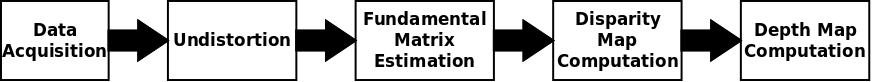
\includegraphics[scale=.3]{images/overview.png}
\caption{Overview of the entire algorithm.}
\label{fig:overview}
\end{figure}

\section{Data acquisition}

Although it might seem as the easiest step of this project, this has to be done very carefully because it has a huge impact on the quality of the results. In other words, algorithms used later cannot handle every situations so we need to capture images that respect many constraints. 

\subsection{Camera calibration}

First of all, I calibrated each camera to obtain the camera calibration matrix and distortion coefficients. This step cannot be avoided because the cameras have a fish-eye lens which causes huge distortion on the images.
I ran a software based on the example provided by the OpenCV tutorials\footnote{http://docs.opencv.org/doc/tutorials/calib3d/camera\_calibration/camera\_calibration.html} which itself is based on \cite{calib2000}. Every tenth of a second, the software is looking for a chessboard in the current image. If it finds it, it will extract points from the images. This step must to be done at least ten times to provide good results. A higher number of points will help getting good results and I did it 25 times. From a set of points, I use functions provided by the OpenCV library to compute the camera calibration matrix and distortion coefficients. This allows to undistort images, which simplifies computations of the fundamental matrix. The effect of undistortion is shown in figure~\ref{fig:distorted-undistorted}.

\begin{figure}[htbp]
    \centering
    \begin{minipage}[c]{.4\linewidth}
        \begin{center}
            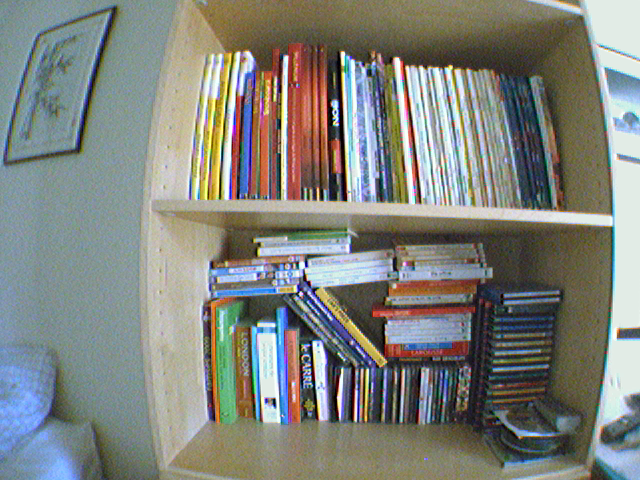
\includegraphics[scale=.25]{images/distorted.png}
        \end{center}
    \end{minipage}
    \hfill
    \begin{minipage}[c]{.4\linewidth}
        \begin{center}
            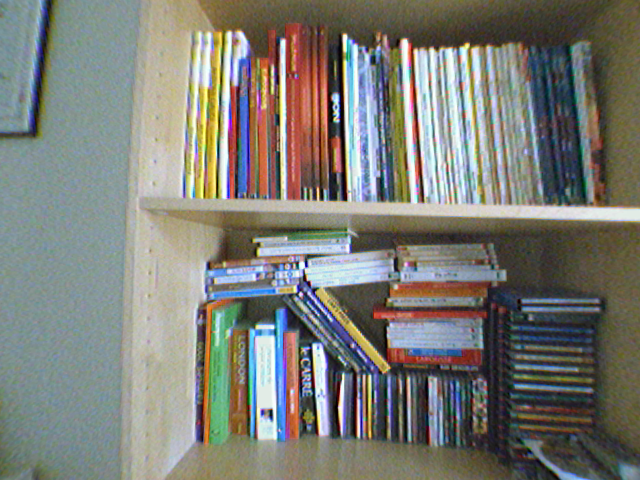
\includegraphics[scale=.25]{images/undistorted.png}
        \end{center}
    \end{minipage}
    \caption{Distorted and Undistorted images}
    \label{fig:distorted-undistorted}
\end{figure}

Notice how corners of the distorted images are not appearing in the undistorted image. This allows some flexibility while capturing images (e.g. one corner of the image can be saturated or too dark without having any effects on the results).

\subsection{Constraints when capturing images}

The quality of the results depends a lot on the input because each piece of hardware and each algorithm have some constraints. Hence, it is necessary to choose a scene with care because it will have a lot of impact later. 

\paragraph{Cameras} They cannot handle high contrast in the image. For outdoors scene, this is a major problem because there is often a lot of contrast between objects directly lit by the sun and shadows. Hence, some parts such as the sky or reflective surface are too saturated. Also, when camera are moving, the image is blurry because the exposure time is too high. Unfortunately, lowering the exposure time would make the image too dark.
\paragraph{Computer}
 Using a desktop computer means that I need a power supply. It also time consuming to install everything before capturing images.
\paragraph{Fire-Wire cable}: I cannot put my cameras far away from the computer. This was a huge cause of trouble because I had to move temporarily the desktop computer to the bedroom of my flat mate to access a small garden each time I wanted to capture scene outdoors.
\paragraph{Feature point detector}: Feature point detectors work well if they are a lot of corners in the image. Plain surfaces such as white walls lead to poor results.
\paragraph{Feature point matching}: Every features detected must be as unique as possible to avoid any mismatch. Since, all algorithms work on set of points correspondence. It is vital that the number of mismatch is very low (less than 5\%). So the scene must not contain any repetitive patterns such as a brick wall or foliages.
\paragraph{Stereo algorithms}: Stereo algorithms impose constraints on the lighting of the scene. Since they often work by comparing pixels from both images, there must be as few shadows as possible. Plain surfaces must also be avoided. Also, the use of artificial lighting must be avoided because it makes sharp shadows. Taking images in daylight is better because shadows are softened.

\subsection{Capturing images}

I implemented a small software which captures frames at 60 frames per second from both cameras and can provide several options such as making a video of the images. I was not able to configure cameras to ensure that both capture frames exactly at the same time. Fortunately, the delay is negligible. I also used coriander, a software which gives access to parameters of cameras. This was very convenient if the scene was not lit correctly.


\subsubsection{Garden}
At the beginning, I started capturing images in a small garden because there would be a few meters between cameras and any other objects. Here are some images:

\begin{figure}[H]
\begin{tabular}{cc}
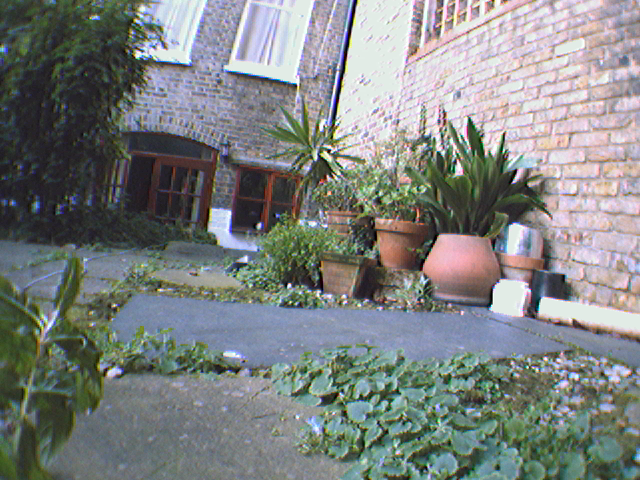
\includegraphics[scale=0.25]{images/garden1_left.png} &
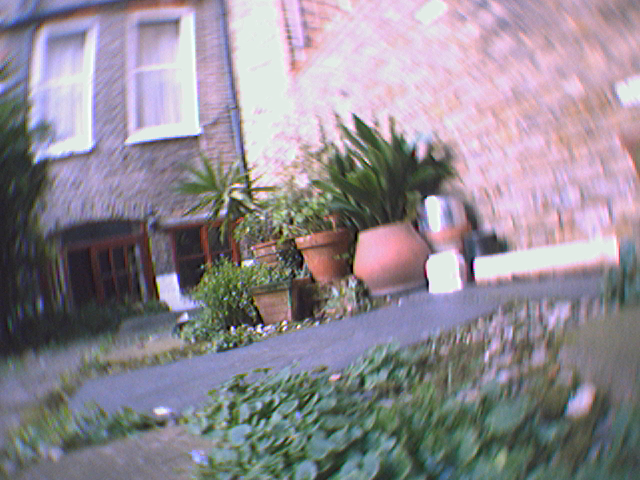
\includegraphics[scale=0.25]{images/garden1_right.png} \\
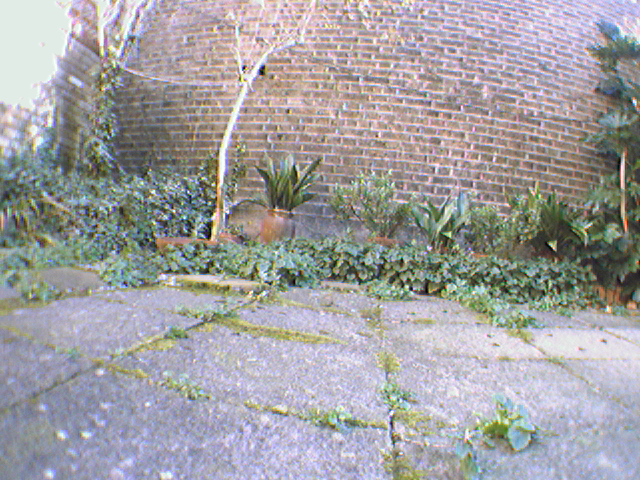
\includegraphics[scale=0.25]{images/garden2_left.png} &
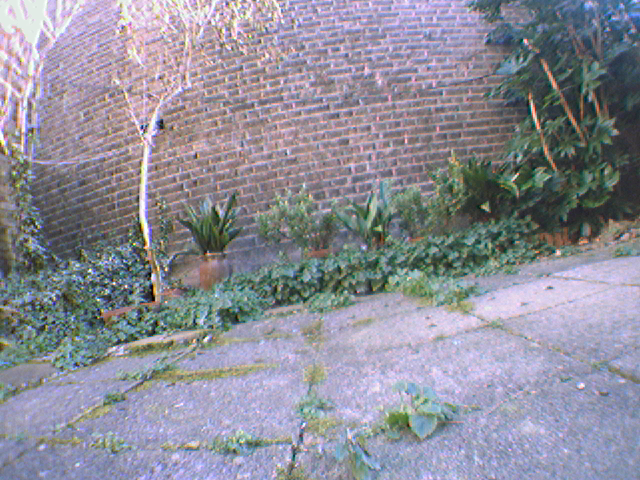
\includegraphics[scale=0.25]{images/garden2_right.png} \\
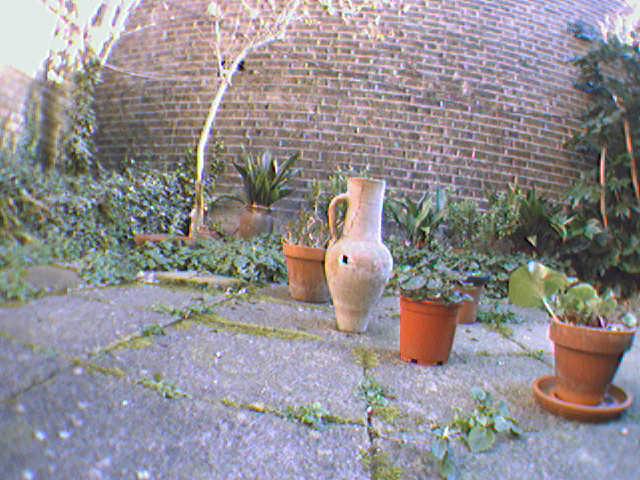
\includegraphics[scale=0.25]{images/garden3_left.png} &
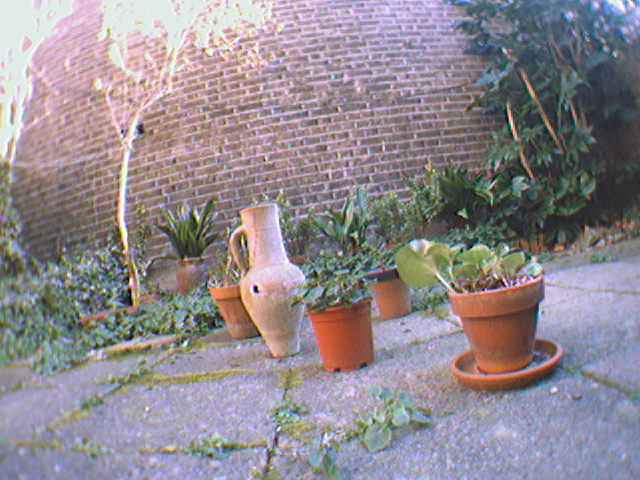
\includegraphics[scale=0.25]{images/garden3_right.png} \\
\end{tabular}
\caption{Images taken in a garden}
\end{figure}

All feature point matching algorithms provided by OpenCV failed to work with these images. Even though it is able to detect many features in these images, especially in foliages and walls, it is not able to match correctly many features because each feature is not unique. For instance, the corner of a brick is a good candidate for a feature point. However, all features corresponding to corners of bricks have a very similar feature descriptor. If feature point matching is very strict about 
The percentage of mismatch is very high so these data sets are unusable.

\subsubsection{Shelves}

After many attempts in the garden, I decided not to capture frames outdoors. I imitated the tsukuba scene, two tests images used for testing the quality of disparity map produced by stereo algorithms.

\begin{figure}[H]
\begin{tabular}{cc}
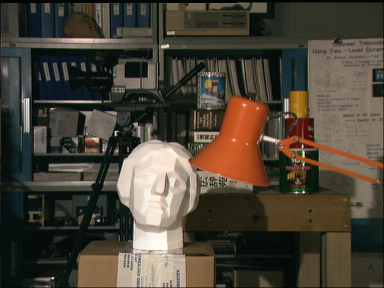
\includegraphics[scale=0.45]{images/tsukuba_left.png} &
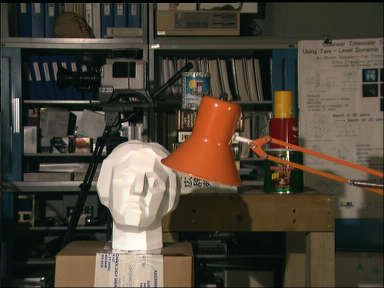
\includegraphics[scale=0.45]{images/tsukuba_right.png} \\
\end{tabular}
\caption{Tsukuba scene}
\end{figure}

I chosed to capture two shelves full of books, comic strips and cd cases. Corner of these objects are very good candidate for feature points and feature matching works well. I payed attention about lighting to minimise shadows below the shelves and I also had to adjust the amount of light in the room such that I did not need to change the default exposure time.

\begin{figure}[H]
\begin{tabular}{cc}
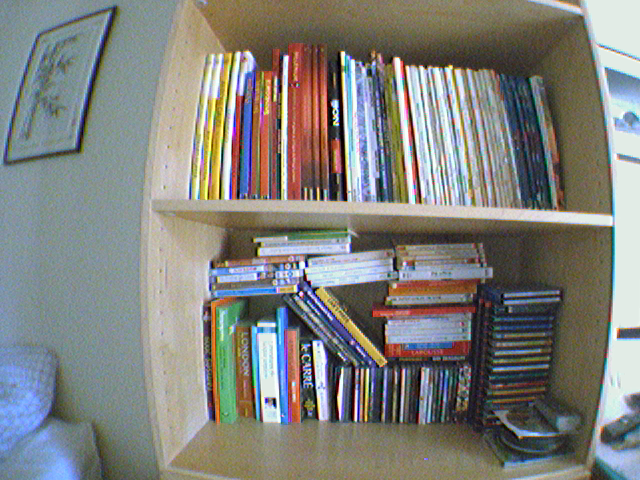
\includegraphics[scale=0.25]{images/shelves_left.png} &
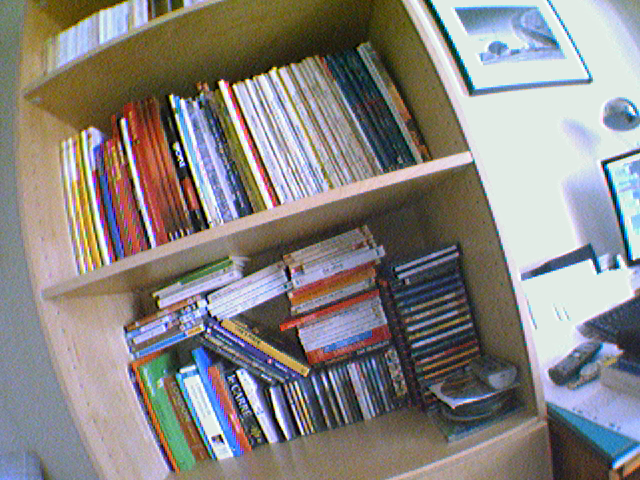
\includegraphics[scale=0.25]{images/shelves_right.png} \\
\end{tabular}
\caption{Shelves}
\end{figure}

This dataset contains 200 pairs of images taken at 60 images per second. The left camera is still while the right camera moves. I will always refer to this dataset as \textbf{shelves}.

These images respect most contrainsts described above. However, there are some troubles:
\begin{enumerate}
    \item Most points lie on the same plane. This is the worst situation for RANSAC because it will often finds invalid solutions.
    \item I forgot to slightly diminish the exposure time of the cameras. While moving the right camera often captures blurry images. For this reason, 26\% images of the dataset are blurry and should produce bad results.
    \item There are still some shadows below the shelf.
    \item For one data set, I forgot to place an object in front of the shelves.
    \item Most feature points are localised in the center of the image.
\end{enumerate}

\subsubsection{Poster}

I bought a poster on placed it on a white wall near a window for good lighting. I placed my cameras at 90 centimetres from the ground, facing the poster at a distance of 130 centimetres.

\begin{figure}[H]
\begin{tabular}{cc}
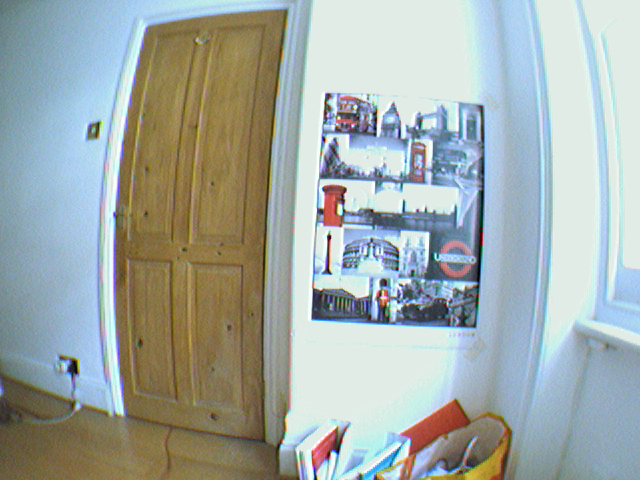
\includegraphics[scale=0.25]{images/poster_left.png} &
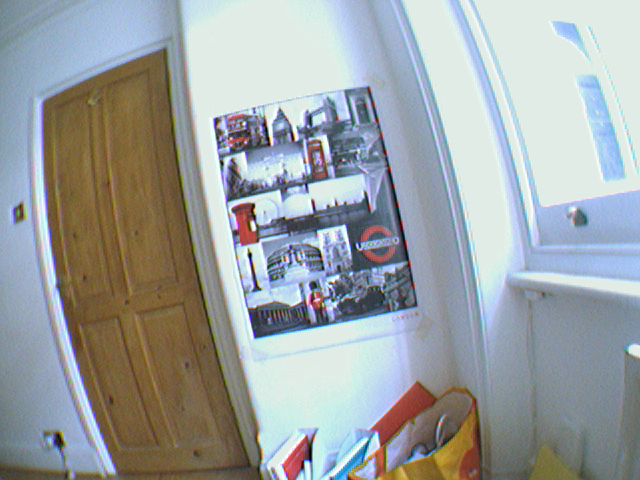
\includegraphics[scale=0.25]{images/poster_right.png} \\
\end{tabular}
\caption{Shelves}
\end{figure}

Like the dataset shelves, the dataset \textbf{poster} contains 200 pairs of images.

Feature point detectors and matching work very well with these images. It only detects feature points from the poster and nowhere else. This is not a problem because it detects enough points correspondences. However, white walls are a problem during the computation of the disparity map.

\subsection{Model computation}

To take into account the deformation of the plate later in the computation of the fundamental matrix and in the metric scene reconstruction, we need to understand how the right camera moves relative to the left camera. The computation of the model depends on the Mecchano structure. I made a first structure but I did not collect data to describe this model, and then I did some slight modifications. Unfortunately, it means that I am not able to use the model described while using the dataset shelves.


The model describes how the $x$ and $y$ components of the translation vector as well as its length varies according to the angle $\theta$ of the right camera. In other words, a model is a list of functions: $f_x(\theta)$, $f_y(\theta)$ and $f_s(\theta)$.

\begin{figure}[H]
    \begin{center}
        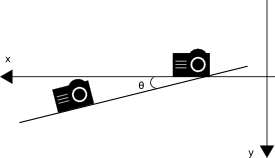
\includegraphics[scale=0.4]{images/modeltheta.png} 
        \label{fig:theta}
        \caption{Angle $\theta$}
    \end{center}
\end{figure}

Notice that we define the y axis downwards to be consistent with the OpenCV library.
\\
To obtain data to create this model, I started by setting my smartphone parallel to the cameras, approximately 30 centimetres from them. I took a video while I was bending the plate. Then, for every other frame of the video, I clicked on six different points to create 3 vectors as shown in figure \ref{fig:model-software}:

\begin{figure}[H]
    \begin{center}
        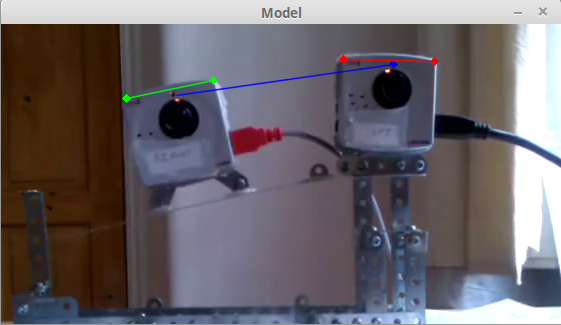
\includegraphics[scale=0.6]{images/model-software.png} 
        \label{fig:model-software}
        \caption{Software to obtain data}
    \end{center}
\end{figure}

From red and green vectors, one could compute the bending angle $\theta$ and the blue vector was used to get x and y coordinates.
I computed a linear and a quadratic approximation for both $f_x$ and $f_y$.

\begin{figure}[H]
    \begin{center}
        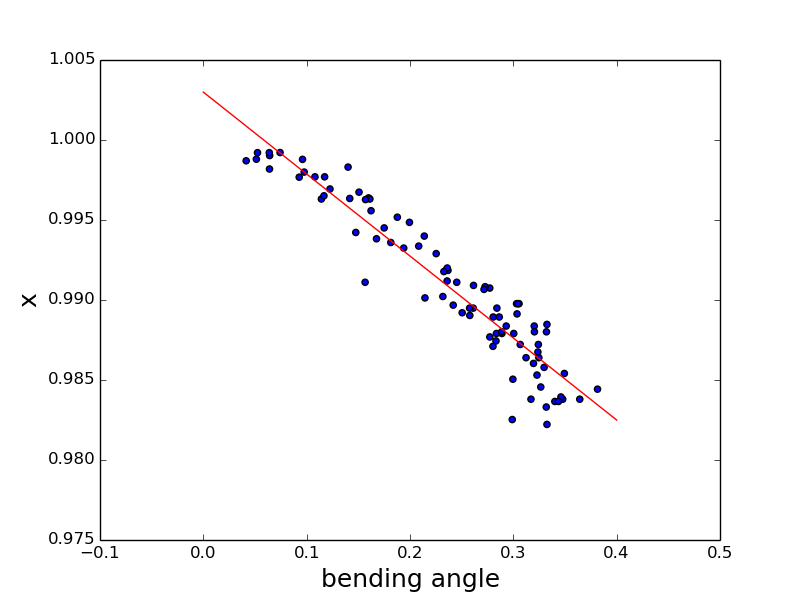
\includegraphics[scale=0.5]{images/model-linear-x.png}
        \label{fig:newmodelX}
        \caption{Approximation of $f_x(\theta) = a\theta + b$}
    \end{center}
\end{figure}

\begin{figure}[H]
    \begin{center}
        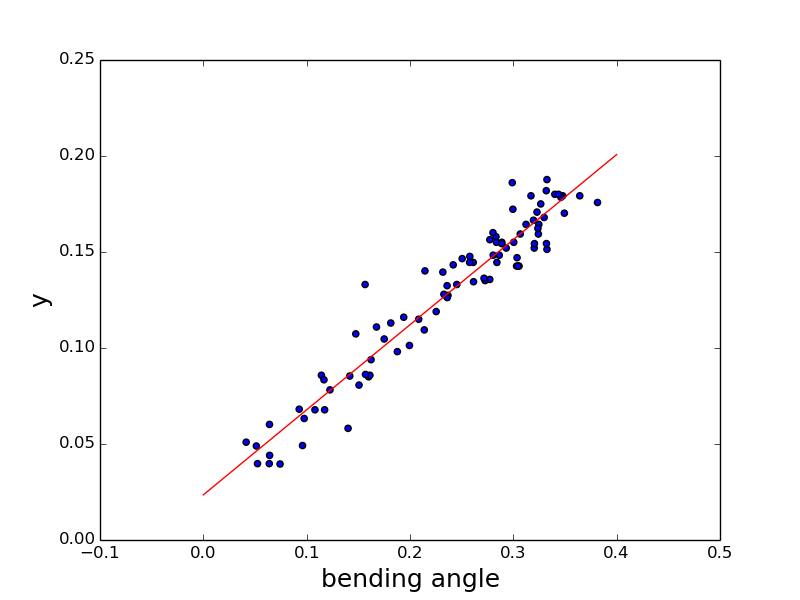
\includegraphics[scale=0.5]{images/model-linear-y.png}
        \label{fig:newmodelY}
        \caption{Approximation of $f_y(\theta) = a\theta+b$}
    \end{center}
\end{figure}

Notice how $f_y$ is very close to the identity function.

\begin{figure}[H]
    \begin{center}
        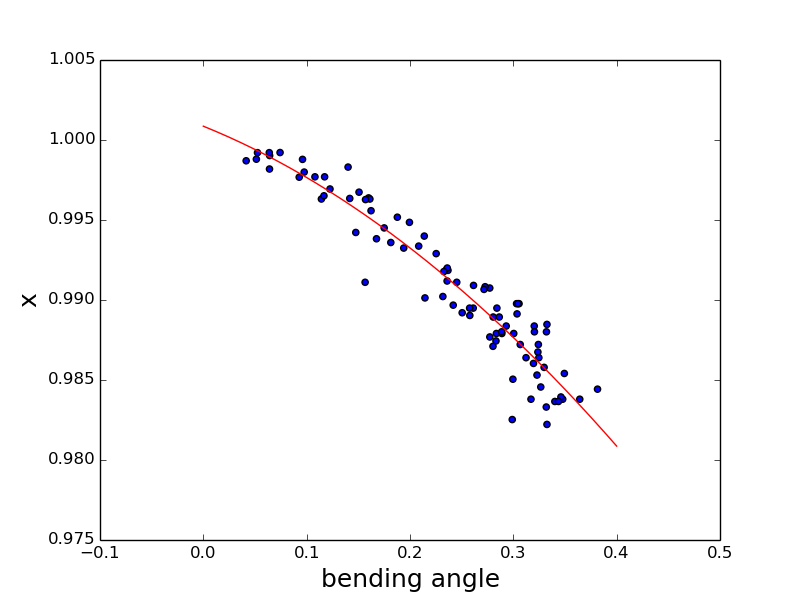
\includegraphics[scale=0.5]{images/model-quadratic-x.png}
        \label{fig:newmodelX}
        \caption{Approximation of $f_x(\theta) = a\theta^2 + b\theta + c$}
    \end{center}
\end{figure}

\begin{figure}[H]
    \begin{center}
        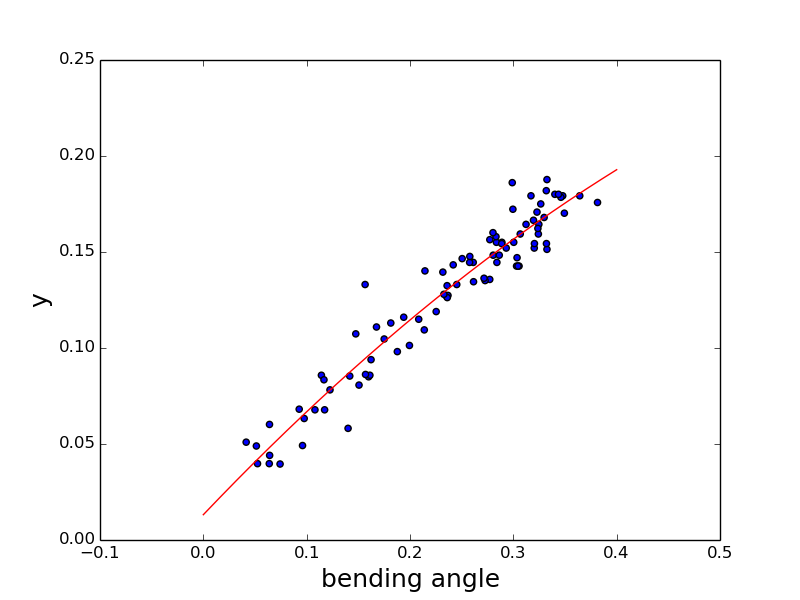
\includegraphics[scale=0.5]{images/model-quadratic-y.png}
        \label{fig:newmodelY}
        \caption{Approximation of $f_y(\theta) = a\theta^2 + b\theta + c$}
    \end{center}
\end{figure}

Concerning $f_s$, a linear model was considered sufficient

\begin{figure}[H]
    \begin{center}
        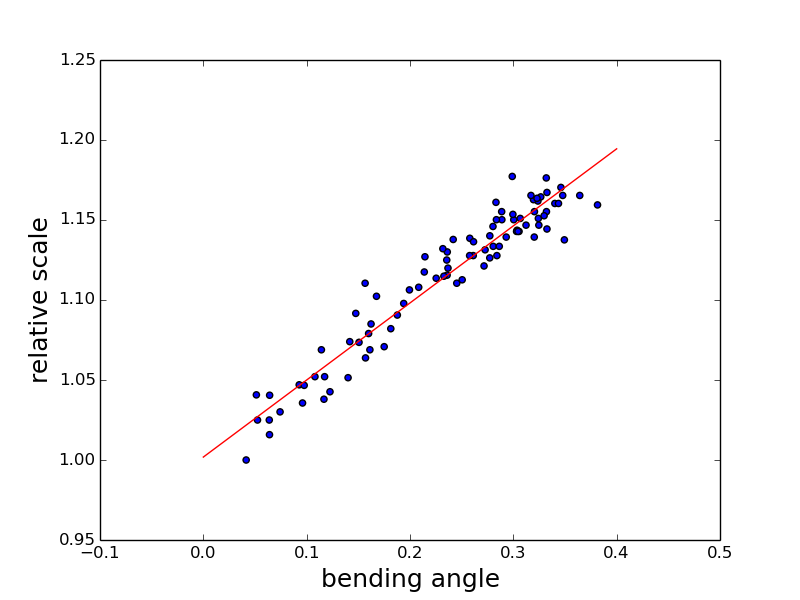
\includegraphics[scale=0.5]{images/model-scale.png}
        \label{fig:newmodelS}
        \caption{Approximation of $f_s(\theta) = a\theta+b$}
    \end{center}
\end{figure}

$f_s$ describes how the scale varies given the bending angle $\theta$. I defined $f_s$ such that for the minimal angle $\theta_{min}$, $f(\theta_{min}) = 1$. Figure \ref{fig:newmodelS} shows that the scale does not vary more than 20\% while the bending angle is at its maximum. This function is not sufficient to recover the real distance between both cameras because it is still up to scale.

\section{Detecting points correspondence}

Detecting enough points correspondences is vital for obtaining a result at the end because most algorithms used in this project do not perform directly on images but rather on points correspondences. First, feature detectors computes a list of features in both images as well as their descriptor. Then, feature point matching associates features belonging to different images, thus creating a list of points correspondence. Ideally, this step should be as fast as possible while having a very low number of mismatch.
I use feature point detectors provided by the OpenCV library. I have a choice of two algorithms: SURF, ORB. Others are available. To evaluate each feature detector, I run it against the shelves dataset. To improve spatial distribution of the feature point detection, I split each image into four parts and run the feature point detection and matching algorithm on each part. For each algorithm, I selected parameters that gave the best results while guaranteeing a minimum of 200 matches for each pair of image. We also need to take into account the number of matches detected because detecting and matching more points take more time.

\begin{figure}[H]
\centering
\begin{tabular}{|c|c|c|}
\hline
& \shortstack{\\SURF \\ (minHessian=5810, \\ distance=35)} & \shortstack{\\ORB \\ (nbFeatures=500, \\ distance=35)} \\
\hline
average number of match & 266.825 & 1991.81 \\
\hline 
average time & 619.7ms & 179.452ms \\
\hline
average time per match & 2.32249ms & 0.090095ms \\
\hline
\end{tabular}
\caption{Comparing SURF and ORB}
\end{figure}

From these figures, ORB is much faster than SURF. Evaluating the percentage of mismatch is harder to measure because I cannot compute a list of true points correspondence. One simple way to is to view these feature points. If the algorithm works well most lines joining two feature points are parallel because feature points all lie on the same plane. Here is one example with SURF and ORB:

\begin{figure}[H]
\begin{tabular}{c}
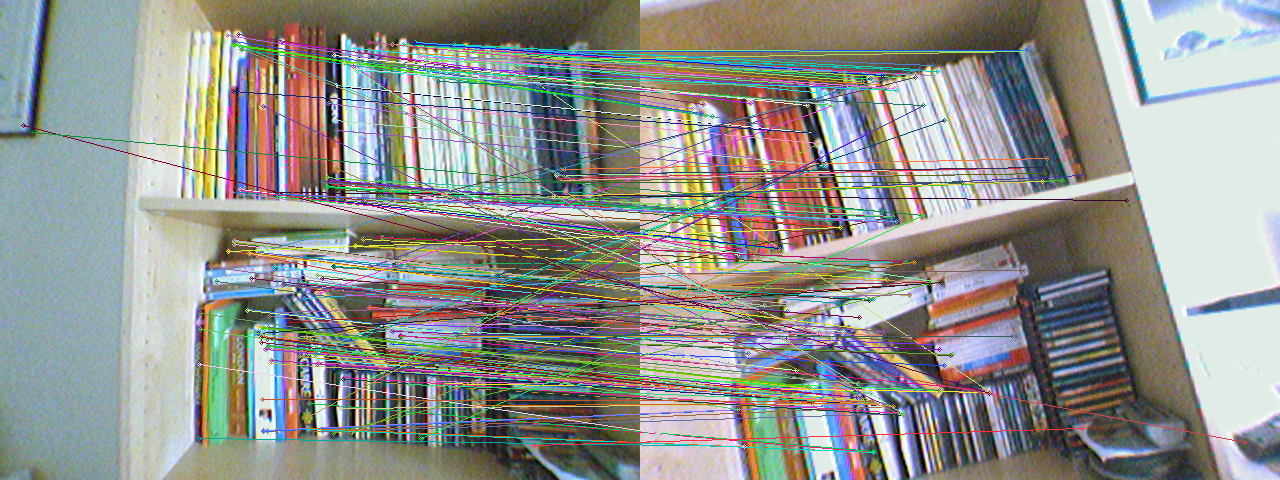
\includegraphics[scale=0.3]{images/surf_bad.png} \\
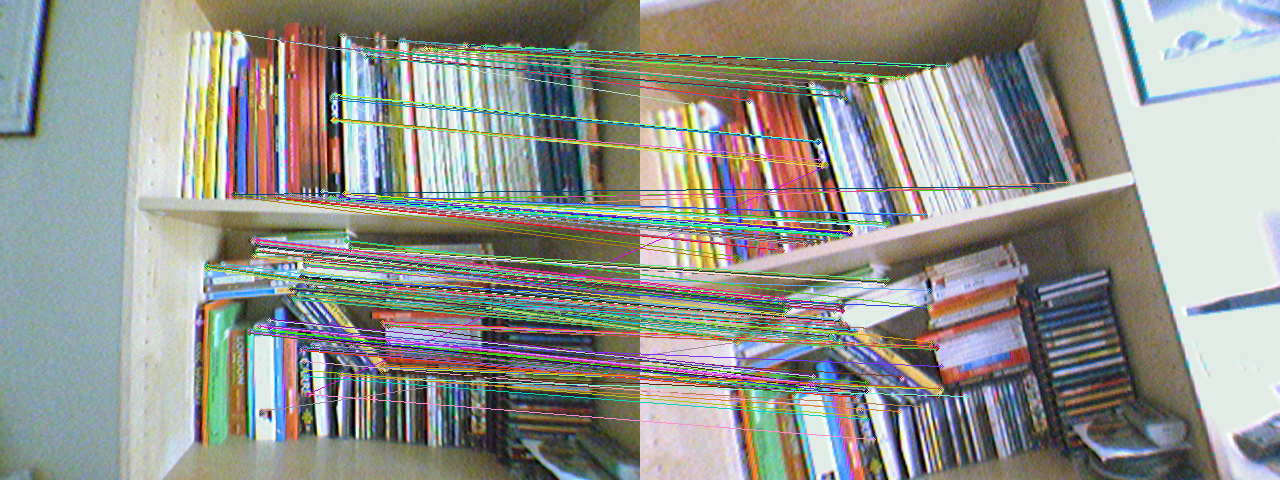
\includegraphics[scale=0.3]{images/orb_good.png} \\
\end{tabular}
\caption{Top: SURF(minHessian=5810, distance=35). Bottom: ORB(nbFeatures=500, distance=35).}
\end{figure}

SURF does not perform as well as ORB. Another way to compare both algorithms consists in computing a very accurate fundamental matrix given a pair of images using different means, then compute the re-projection error for each point correspondence. The distribution of errors have a larger standard deviation if the feature detector and matching does not work well because mismatch have bigger re-projection errors compared to correct matches.

For this project, the default method for detecting points correspondence is sum up in Algorithm \ref{algo:points}.

\begin{algorithm}[H]
    \KwIn{Left and right images}
    \KwOut{list of points correspondences}
    Split both images in four\;
    Apply ORB(nbFeatures=500, distance=35) on each part\;
    Merge four pairs of lists\;
    Apply feature point matching to create list of points correspondences\;
  \caption{Algorithm for detecting points correspondences}
  \label{algo:points}
\end{algorithm}

\section{Initial guess with RANSAC}

To compute a first approximation of the fundamental matrix given a pair of image, I tried several variants of RANSAC \cite{Ransac81}. This step requires a significant number of correct points correspondence, at least a hundred.

\subsection{RANSAC - OpenCV}

The OpenCV library provides a deterministic implementation of RANSAC which relies on the eight-point algorithm to compute the fundamental matrix from a sample. Two parameters can be set: a threshold $t$ and the level of confidence(i.e. the probability $p$ that the result is correct). The default value of $p$ is 0.99. I never changed this parameter. The OpenCV library sets parameter $t$ to 3 by default. Care must be taken while choosing this parameter. Increasing the threshold too much would mean that all points correspondences are inlier. RANSAC would not be able to discriminate results. On the other hand, if the threshold is too low only points lying on the same plan will be considered as inlier. This leads to degenerate configuration.

Unfortunately, while running with the dataset shelves this implementation of RANSAC, I found that it is very sensitive to the threshold value:

\begin{figure}[H]
	\centering
	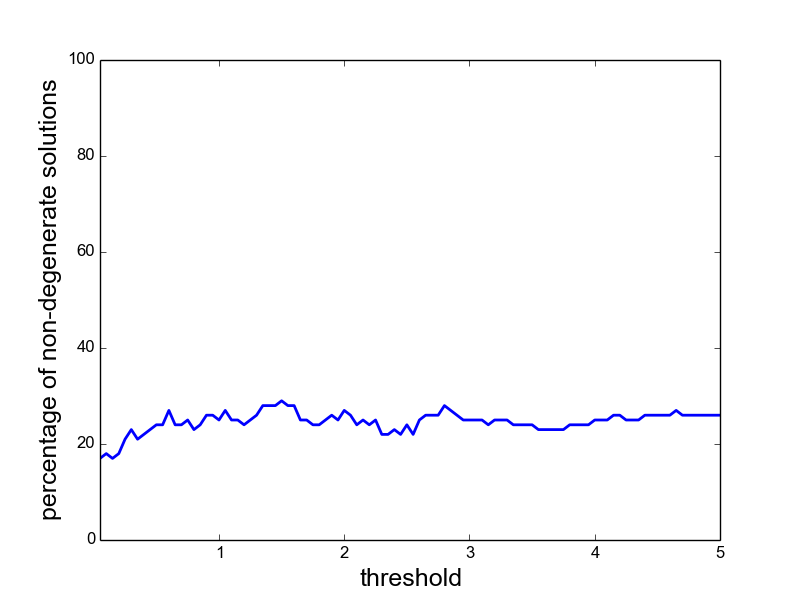
\includegraphics[scale=0.7]{images/ransac-t.png}
    \caption{Percentage of non-degenerate solutions depending on threshold $t$}
    \label{fig:ransac-treshold}
\end{figure}

Notice that when the threshold is in the range 4.8--5, the curve is flat. This means that all points are considered inlier so RANSAC always returns the same solution regardless of the threshold.

In practice, I must manually find the best threshold for each pair of image, otherwise the algorithm will work only in a few cases. In the case where it does not work, RANSAC returns correct solutions from a mathematical point of view (i.e. the solution which minimises $x'^\top Fx$) but which are invalid with regards to the reality. For instance, the following image shows an example of an incorrect result:

\begin{figure}[H]
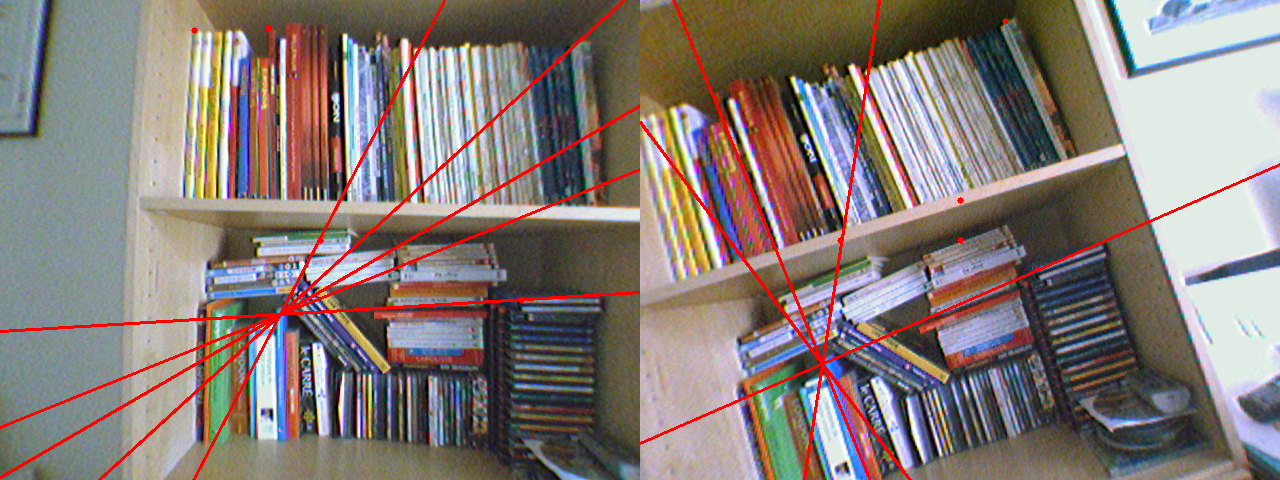
\includegraphics[scale=0.3]{images/degenerate.png}
\caption{Example of a degenerate configuration}
\end{figure}

Notice that the epipoles are projected on the image, at the intersection of the epipolar lines. It would mean that the right camera is looking at the left camera which never happened during this project.

\subsection{RANSAC-N}

A solution to this problem is to run $N$ times RANSAC with different parameters. Either we can either change the threshold $t$ or the distance parameter $d$ of the feature point matching algorithm. I only tried to change one parameter while the other was constant. It might have been better to explore all combinations $(t, d)$ to minimise $N$.

Then, we need algorithms for:
\begin{enumerate}
    \item Detecting invalid solutions.
    \item Selecting best fundamental matrix out of the valid solution set.
\end{enumerate}

\paragraph{Detecting degenerate configuration} I project both epipoles and check whether it would be visible in the image. This test assumes that the epipole should project far away from the center of the image because both cameras are nearly coplanar. One drawback is that it may happen that the epipole project close to the border of the image and yet still considered as a valid solution.

\paragraph{Method for selecting best solution} One could choose the fundamental matrix which gives the minimal re-projection error. This minimises the disparity between the left and right image during image rectification. Other choices are possible such as the distance of the projected epipolar line to the center of the image. This favours solutions which minimises the distortion during the image rectification step because it reduces the angle between epipolar lines (appearing as more parallel in the image) corresponding to features in the image. In practice, the former solution produces a disparity map with less noise and thus it is the preferred choice for selecting solutions.

Alternatively, a two-in-one algorithm consists in rectifying images for each possible solution and count the percentage of black pixels in rectified images. Here, we seek to fill the rectified images as much as possible such that stereo matching algorithms avoid working with invalid data.

\begin{comment}
\begin{algorithm}[H]
  \KwIn{List of points correspondence}
  \KwOut{Fundamental matrix F}
  \For{i from 1 to N} {
    $F_i$ = RANSAC(t, points)\;
    \If{$e_i$ or $e'_i$ projects to the image}{
      Discard $F_i$\;
    }
  }
  Select $F_i$ which has the minimal re-projection error\;
  \caption{Algorithm to cope with RANSAC }
\end{algorithm}
\end{comment}

\subsubsection{Modifying threshold}

The threshold depends on how precise each point has been detected by the feature point detector. Based on figure~\ref{fig:ransac-treshold}, a sensible range to explore would be 0.05--5 with increment of 0.05. The feature point detection and matching is performed with the usual parameters.

I wrote a program to find a set of threshold such that RANSAC can find at least one valid solution for the entire dataset. This algorithm does not guarantee to find the minimal $S$. First, each candidate threshold $t$ is associated with a set of indices which represents the set of valid solutions produced by RANSAC using this candidate. Then, the threshold associated with the largest set of indices is added to the solution set $S$ and removed from the candidate set. In an iterative manner, a score is computed for each candidate left. This score represents the number of indices which is associated with this threshold but is not associated with any thresholds in $S$. The threshold with the highest score is inserted in $S$ and removed from the candidate set. This step is repeated until all indices are associated with at least one threshold in $S$ or the maximum score is equal to zero.

This gives the following set of thresholds for the dataset shelves:
\begin{center}
\begin{tabular}{|c|c|c|c|c|c|c|c|c|c|}
\hline
$t$ & 1.5 & 0.6 & 4.05 & 1.05 & 0.05 & 0.1 & 1.9 & 0.2 & 0.4  \\
\hline
score & 58 & 25 & 19 & 9 & 6 & 5 & 5 & 4 & 3 \\
\hline
$t$ & 2.65 & 0.8 & 0.15 & 0.65 & 1 & 1.35 & 1.55 & 1.85 & 2.25 \\
\hline
score & 2 & 1 & 1 & 1 & 1 & 1 & 1 & 1 & 1\\
\hline
\end{tabular}
\end{center}

To reduce computation time, I discarded the last seven thresholds. I can compute a non-degenerate solution for 69.5 \% of the dataset shelves.

\subsubsection{Modifying distance}

In this case, we let the threshold unchanged to its default value but varies the distance parameter of the feature point matching algorithm. This means that some inputs will have a low probability to contain mismatch but the number of feature points might be too low. Another solution would be to vary the threshold parameter of RANSAC instead.
I chose empirically the range of the parameter to explore by determining the minimal value such that sufficient points correspondence are found in each pair of image of the dataset. I computed the percentage of non-degenerate solutions over the range 30--80:

\begin{figure}[H]
	\centering
	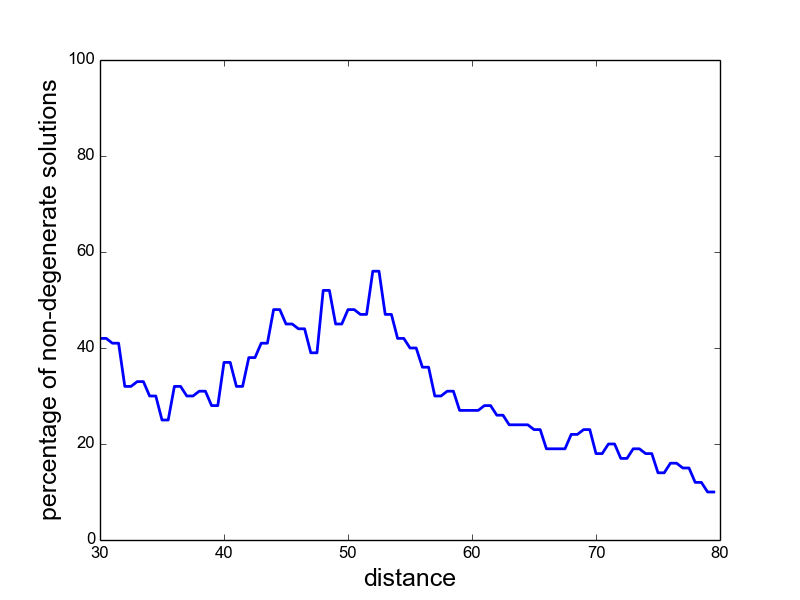
\includegraphics[scale=0.7]{images/ransac-d.png}
    \caption{Percentage of non-degenerate solutions depending on distance $d$}
    \label{fig:ransac-distance}
\end{figure}

From \ref{fig:ransac-distance}, it is clear that a distance above 55 leads to more mismatch and thus higher probability to find a degenerate solution.
I used the same algorithm than previously to find the minimal solution $S$:

\begin{center}
\begin{tabular}{|c|c|c|c|c|c|c|c|}
\hline
d & 52 & 44 & 36 & 48 & 31 & 45 & 37 \\
\hline
score & 113 & 43 & 21 & 12 & 7 & 3 & 1 \\
\hline
\end{tabular}
\end{center}

In the end, we are able to find a non-degenerate solution for the entire shelves dataset.

\subsection{QDEGSAC}

To avoid running multiple times RANSAC, I looked at the existing literature about modifying RANSAC to deal with degenerate solutions. One idea is to filter out points correspondences that cause degenerate solutions. This approach was taken by QDEGSAC~\cite{Qdegsac06} and Plunder~\cite{Plunder95}. I implemented QDEGSAC as defined in the paper. With default parameter settings, I found that it was able to find a non-degenerate solution for 39\% of the dataset. I suspect there might be a bug in my implementation.

\subsection{RANSAC - OpenGV}

The OpenGV library provides an  implementation of RANSAC based from \cite{Ransac97}. Unlike the implementation from OpenCV, this one is non deterministic. Moreover, the definition of the threshold is slightly different than previously\footnote{http://laurentkneip.github.io/opengv/page\_how\_to\_use.html}. OpenGV relies on the reprojection error to classify points as inlier or outliers. The threshold cannot be a distance in pixels instead it becomes:

\begin{equation}
\epsilon_threshold = 1 - cos(arctan(\frac{\psi}{l}))
\end{equation}

where $\psi$ is the reprojection error in pixels and $l$ is the focal length. 

In addition, this library lets me have a choice of four algorithm to compute the fundamental matrix from a sample of the dataset:
\begin{itemize}
  \item 5-point algorithm by Nist\'er \cite{FivePointNister04}
  \item 5-point algorithm by Stewenius \cite{fivepointstewenius}
  \item 7-point algorithm 
  \item 8-point algorithm
\end{itemize}

I did not use the last two algorithms for two reasons. First of all, there generate more often degenerate solutions compared to the 5-point algorithms. Secondly, they require about an order of magnitude more iterations in RANSAC. I could not find major differences between the two variants of the 5-point algorithm. I only used the 5-point algorithm by Stewenius during this project. The choice of the threshold is crucial for obtaining consistently non-degenerate results but unlike the previous implementation it is much less sensitive and could be set to a fixed value while RANSAC was operating on the entire shelves dataset. I set $\psi = \frac{\sqrt(2)}{2}$.

\section{Model rectification}

After performing RANSAC, the fundamental matrix $F$ is decomposed into a rotation matrix $R$ and a translation vector $T$. Both the translation vector and the rotation matrix are transformed. Due to the position of the right camera, this translation vector $T=(x,y,z)^\top$ where $x$ should be in the range 0.9--0.99 and $y$ in the range 0.05--023. In theory $z$ should be very close to zero. The bending angle can be computed either using the translation vector as $\theta=atan2(Y,X)$ or by decomposing the rotation matrix $R$. In this case, $\theta = atan2(R_{10}, R_{00})$. I found that using the rotation matrix to compute $\theta$ is more robust.

A new translation vector $T_{rectfied}=(f_x(\theta), f_y(\theta), z')$ is computed. The value of $z'$ is chosen such as $T_{rectified}$ is normalised. The new rotation matrix eliminates angles on the x and y axis. Thus,

\[
  R_{rectified} = 
\left (
\begin{matrix}
  \cos(\theta) & -\sin(\theta) & 0 \\
  \sin\theta) & \cos(\theta) & 0 \\
  0 & 0 & 1 \\
\end{matrix}
\right )
\]

Finally, a new fundamental matrix is computed using equation~\ref{eq:fundamental_matrix}.

\section{Gold Standard method}

The gold standard method is one of the application of the Levenberg-Marquardt algorithm to minimise the reprojection error of the fundamental matrix. 
This is a last step of the algorithm to compute refine the fundamental matrix. However, this algorithm works well only if the error follows a Gaussian. I checked it that it is the case by computing the reprojection error from a set of points correspondence using the first pair of image of the shelves dataset. Because reprojection error cannot be negative, the distribution should follow a half-normal distribution:

\begin{figure}[H]
    \begin{center}
        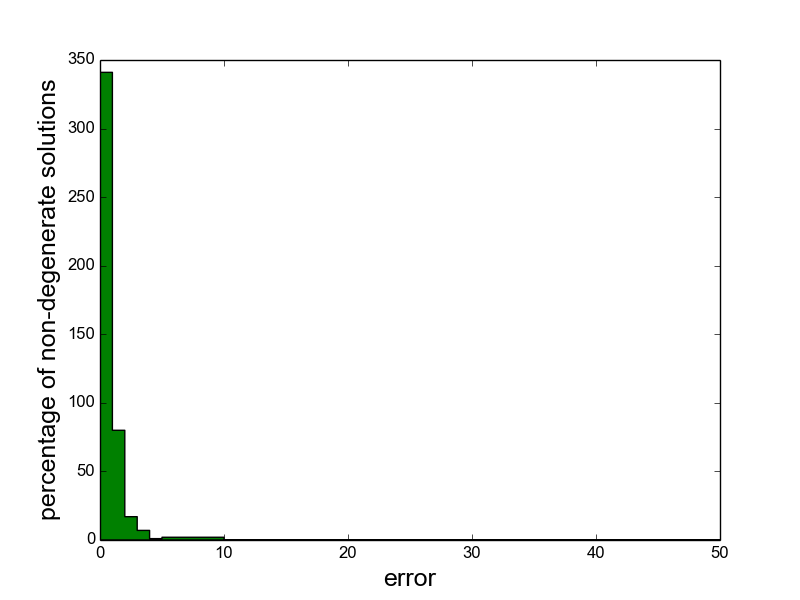
\includegraphics[scale=.45]{images/error_distribution.png}
    \end{center}
    \caption{Error distribution of the reprojection error}
  \label{fig:error_distribution}
\end{figure}

\section{Image rectification}

Image rectification consists in transforming a pair of images such that epipolar lines are parallel to the x-axis (or y-axis). It is necessary to perform this step before the computation of the disparity map because stereo matching algorithms \cite{Stefano02afast} \cite{SGBM} assume that inputs respect this constraint.
I was using the implementation from the OpenCV library but I found that it was either working very well or it failed completely, returning only black images. This was not very convenient as I also wanted to align images even though the result might not be usable  because the fundamental matrix $F$ was not very accurate. I implemented the image rectification algorithm as outlined from the book \textit{Multiple View Geometry in Computer Vision} \cite{Geom}.

The principle of this algorithm is to set the epipoles at infinity. First, we find a homograhy $H'$ for the right image, then we find the homography $H$ for the left image.

A rotation $R$ takes the right epipole $\mathbf{e}'$ to a point on the x-axis. Hence $\mathbf{e}' = (f, 0, 1)^\top$. Then, the matrix $G$ maps this point to the infinity $(1, 0, 0)^\top$. Thus $G$ is defined as:

\[
    \mathbf{G} = \left (
    \begin{matrix}
        1 & 0 & 0 \\
        0 & 1 & 0 \\
        -1/f & 0 & 1 \\
    \end{matrix}
    \right )
\]

In addition, a translation $T$ may change the center of the rotation such that, for instance, the center of the image is not deformed by the image rectification process. Hence, the right homography is:

\begin{equation}
  H' = GRT
\end{equation}

The left homography consists of a product of two matrices:

\begin{equation}
  H = H_AH_0
\end{equation}

where $H_0 = H'M$ and fundamental matrix $F=[\mathbf{e}']_\times M$. We seek to find $H_A$ such that the disparity between the rectified left and right images. Let assume that we have a list of points correspondences $\mathbf{x}_i \leftrightarrow \mathbf{x}'_i$. Furthermore, we define $\hat{\mathbf{x}}_i = H_0\mathbf{x}_i$ and $\hat{\mathbf{x}}'_i = H'\mathbf{x}'_i$.

$H_A$ is of the form :

\[
    H_A = \left (
\begin{matrix}
    a & b & c \\
    0 & 1 & 0 \\
    0 & 0 & 1
\end{matrix}
\right )
\]

such as the values $a$, $b$ and $c$ minimise:
\begin{equation}
    \label{eq:alignment1}
    \sum_i d(H_A\hat{\mathbf{x}}_i, \hat{\mathbf{x}}'_i)^2
\end{equation}

Moreover, $\hat{\mathbf{x}}_i = (\hat{x}_i, \hat{y}_i, 1)^\top$ and $\hat{\mathbf{x}}'_i = (\hat{x}'_i, \hat{y}'_i, 1)^\top$, hence \ref{eq:alignment1} becomes:

\begin{equation}
    \sum_i (a\hat{x}_i + b\hat{y}_i + c - \hat{x}'_i)^2 + (\hat{y}_i - \hat{y}'_i)^2
    \label{eq:alignment2}
\end{equation}

Notice that the term $(\hat{y}_i - \hat{y}'_i)^2$ is constant, so this is equivalent to minimise:

\begin{equation}
    \sum_i (a\hat{x}_i + b\hat{y}_i + c - \hat{x}'_i)^2
    \label{eq:alignment3}
\end{equation}

To find the solution $\mathbf{x} = (a, b, c)^\top$, we use the following algorithm :
\begin{algorithm}[H]
    \KwIn{Matrix A and vector \textbf{b}}
    \KwOut{Solution \textbf{x}}
    SVD A = $UDV^\top$\;
    Set $\mathbf{b}' = U^\top\mathbf{b}$\;
    Build vector $\mathbf{y}$ such that $y_i = b'_i/d_i$ where $d_i$ is the i-th diagonal entry of $D$.\;
    Solution is $\mathbf{x} = V\mathbf{y}$\;
    \caption{Linear least-square algorithm for solving equation $A\mathbf{x} = \mathbf{b}$}
    \label{algo:leastsquare1}
\end{algorithm}

After computing homographies H and H' it is now possible to transform images. Each pixel of the left image at position $(x, y, 1)^\top$ is mapped to $H(x, y, 1)^\top$. Some interpolation is needed to fill the gaps between pixels.

\begin{figure}[H]
\begin{tabular}{cc}
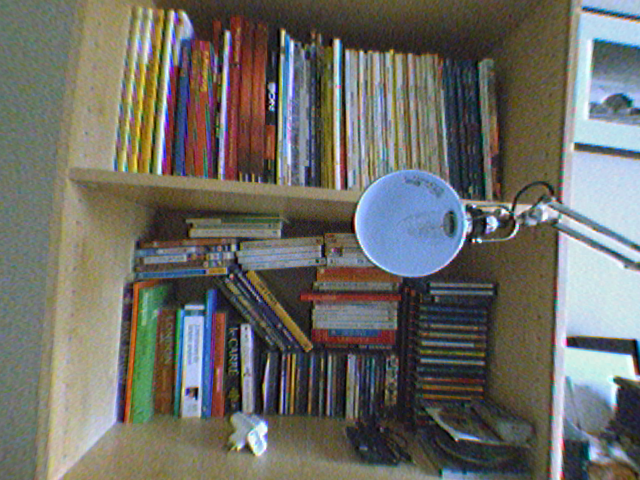
\includegraphics[scale=0.25]{images/unaligned_left.png} &
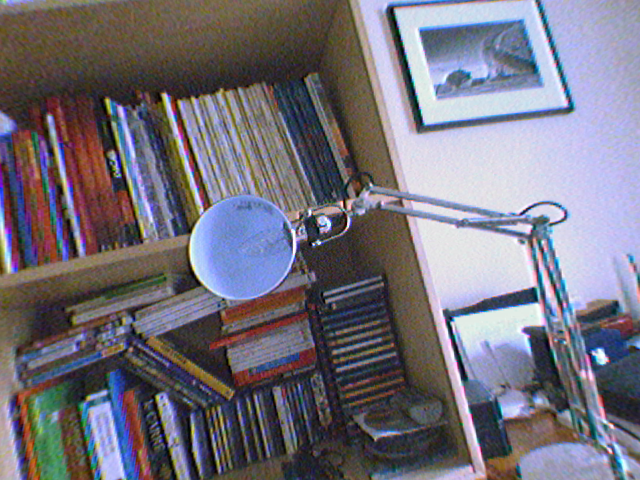
\includegraphics[scale=0.25]{images/unaligned_right.png} \\
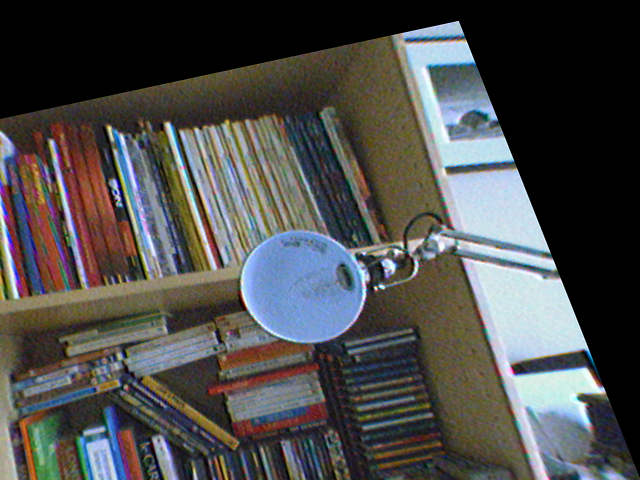
\includegraphics[scale=0.25]{images/aligned_left.png} &
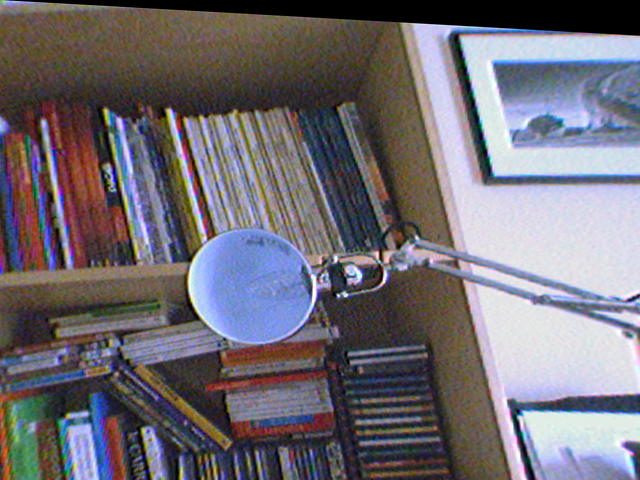
\includegraphics[scale=0.25]{images/aligned_right.png}
\end{tabular}
\caption{Top: Unaligned left and right images. Bottom: Rectified left and right images.}
\end{figure}

The quality of the alignment depends solely on the accuracy of the fundamental matrix $F$. Detecting enough points correspondences for the computation of the left homography is never a problem because if RANSAC runs with success on these images, which needs many points correspondence, this step of the image rectification algorithm cannot fail.

\section{Disparity map and depth map computation}

\subsection{Disparity map}

The disparity map is computed using the semi-global stereo matching algorithm\cite{SGBM} provided by the OpenCV library. The following parameters gave the best results:
\begin{center}
\begin{tabular}{|c|c|}
\hline
\textbf{parameter} & \textbf{value} \\
\hline
minDisparity & 0 \\
\hline
maxDisparity & 64 \\
\hline
SADWindowSize & 7 \\
\hline
disparity smoothness 1 & 1176 \\
\hline
disparity smoothness 2 & 4704 \\
\hline
disp12MaxDiff & 3 \\
\hline
preFilterCap & 0 \\
\hline
uniquenessRatio & 0 \\
\hline
speckleWindowSize & 0 \\
\hline
speckleRange & 0 \\
\hline
\end{tabular}
\end{center}

The output is a $640\times480$ matrix storing disparities as 16-bit signed integer. A value of $-1$ indicates that the algorithm could not find a disparity value. To preview the disparity map, I stored it on disk as a grey-scale image by normalising it using a linear min-max method.

\begin{figure}[H]
    \centering
    \begin{tabular}{cc}
    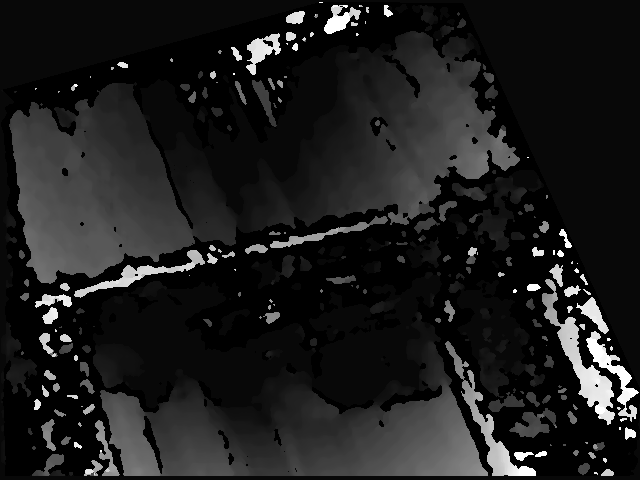
\includegraphics[scale=0.2]{images/disparity_0.png} &
    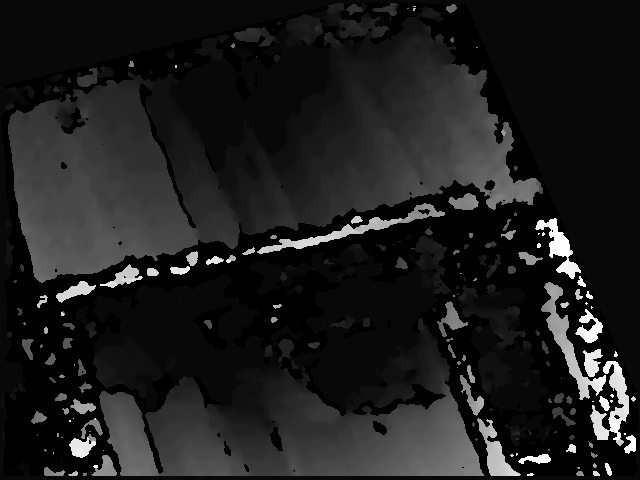
\includegraphics[scale=0.2]{images/disparity_1.png} \\
    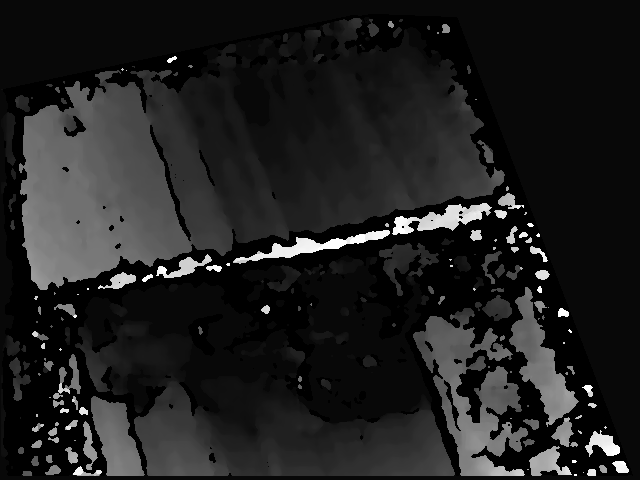
\includegraphics[scale=0.2]{images/disparity_2.png} &
    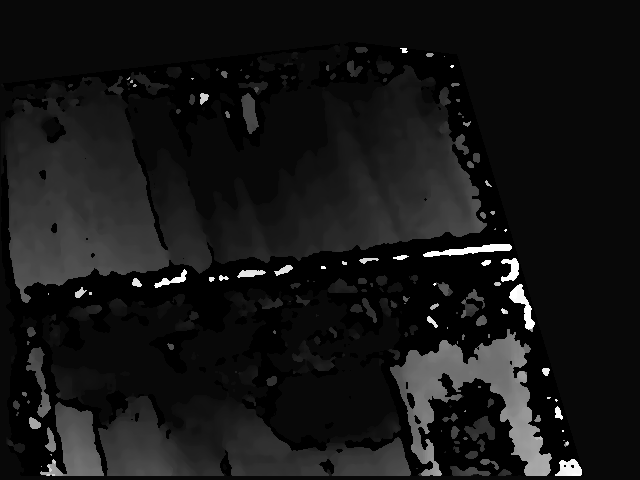
\includegraphics[scale=0.2]{images/disparity_3.png}
    \end{tabular}
    \caption{First four disparities obtained using RANSAC (opengv) and the dataset shelves.}
\end{figure}

\subsection{Depth map}
The depth map is computed from the disparity map using the following equation:
\begin{equation}
  depth = \frac{baseline \times focal length}{\mid disparity\mid} 
\end{equation}

The baseline is expressed in millimetres, thus the depth is also expressed in millimetres. To recover the correct value of the baseline, I have to find the scale factor. This factor depends on the bending angle $\theta$ as shown in figure~\ref{fig:newmodelS}.
Now, all I need is to find the right scale factor for one angle and then compute the baseline as $baseline = s_{min} * f_s(\theta)$. I used two different methods to recover $s_{min}$. 

\paragraph{Method 1:} I set the right camera in the upper position (minimum $\theta$). I placed a chessboard in front of both cameras and I took 25 pairs of images of this chessboard in different positions. This gives a list of points correspondences to compute the fundamental matrix using RANSAC. In addition, each square of the chessboard has a size of $23.7\times23.7mm$. Using this knowledge, one can re-project the points and find the right scale such as the distance between 3D points is $23.7$. I used the implementation provided by OpenCV to compute a fundamental matrix with the right scale. The baseline is the norm of the translation vector. I found a baseline of $122.4$ compared to a measured value of 127.5 (4\% difference) with a decimeter.

\paragraph{Method 2:} I placed both cameras in front of a poster at a distance of 130 centimetres. Furthermore, the feature point detector only detects points belonging to this poster. So all points correspondences lie in a plane. I use the implementation of RANSAC from the OpenGV library to obtain the estimated transformation. However, I cannot use the translation vector because it often returns a degenerate solution regardless of the algorithm used. Fortunately, the rotation matrix is estimated with sufficient accuracy and remains constant (i.e. running multiple times RANSAC leads to the same rotation matrix). I decompose it into cardan angles to get $\theta_x$, $\theta_y$ and $\theta_z$. I use $\theta_z$ and the model described earlier to compute a new normalised translation vector. Then, I triangulate all points correspondences using the new translation vector and the rotation matrix obtained from RANSAC. I compute $z_{avg}$ which represents the average of the $z$ component of all 3D points. The scale $scale_\theta$ is obtained using the following equation:

\begin{equation}
  scale_\theta = \frac{1300}{z_{avg}}
\end{equation}

Notice that $scale_\theta$ may be different than $s_{min}$ because I did not set the right camera in the upper position unlike method 1. In the end, I find a scale of 138 for $\theta_z = 0.26$ radian (approximately \ang{15}). According to figure \ref{fig:newmodelS}, $s_{min} = \frac{138}{f_s(\theta_z)} \approx 115.7$. There is a 9\% difference between the estimated value and the measured value of 127.5. Hence, this method is less precise than the previous one.

Here are the images taken by the left and right camera. The poster is attached to a white wall. After undistortion, only the poster and the wall is visible that's why all points belong to the poster.
\begin{figure}[H]
\centering
\begin{tabular}{cc}
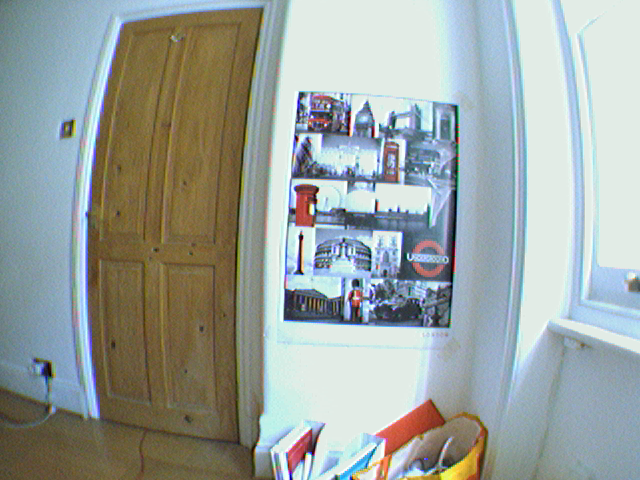
\includegraphics[scale=0.25]{images/left_scale.png} &
o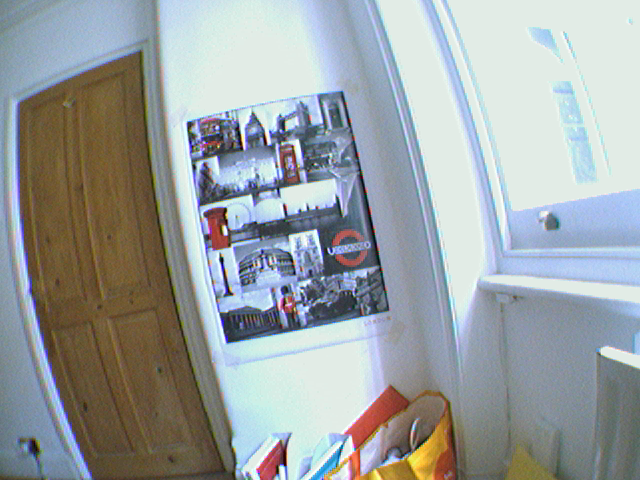
\includegraphics[scale=0.25]{images/right_scale.png} \\
\end{tabular}
\caption{Left \& right images used to compute scale}
\end{figure}

The result of the triangulation is a list of 3D points. As expected, they all lie in a plane:
\begin{figure}[H]
\centering
\begin{tabular}{cc}
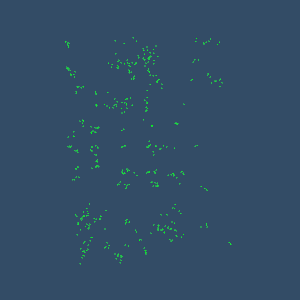
\includegraphics[scale=0.5]{images/cloud1.png} &
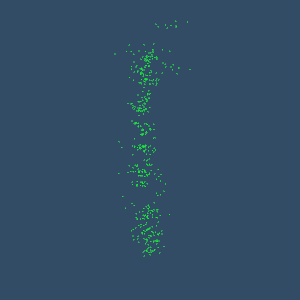
\includegraphics[scale=0.5]{images/cloud2.png} \\
\end{tabular}
\caption{Cloud points viewed from the cameras and from the right side.}
\end{figure}


\chapter{Evaluation}

\section{Model efficiency}

We seek to find out if using a model reduces the reprojection error compared to RANSAC. We assume that the orientation of the right camera is already kwown and is given to the model which computes the translation vector. There are three models to compare: linear, quadratic, and a mixed approach. The last model computes the x component of the translation vector using the quadratic approximation and the y component is computed from the linear approximation. Using the dataset shelves, we compute for each entry of this dataset four different fundamental matrices, with and without model, and compute their respective reprojection error.

\begin{figure}[H]
    \centering
    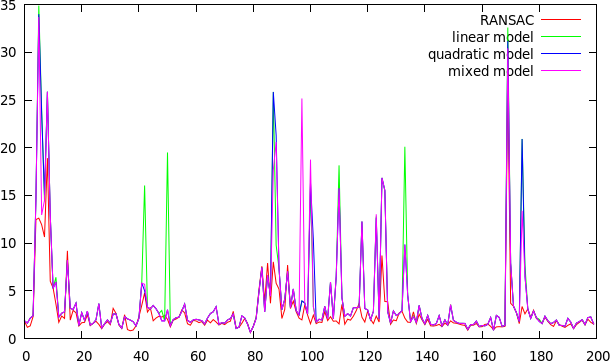
\includegraphics[scale=0.5]{images/error-model.png}
    \caption{Comparison of reprojection error using the shelves dataset}
    \label{fig:error-model}
\end{figure}

From figure \ref{fig:error-model}, it is clear that all models perform similarly to RANSAC at best.

\begin{figure}[H]
\centering
\begin{tabular}{|c|c|c|c|c|}
\hline
& RANSAC & linear model & quadratic model & mixed model \\
\hline
average error & 2.661 & 4.124 & 3.989 & 3.934 \\
\hline
standard deviation & 2.838 & 5.443 & 5.207 & 5.008 \\
\hline
min error & 0.637 & 0.659 & 0.659 & 0.659 \\
\hline
max error & 26.988 & 34.883 & 33.990 & 33.687 \\
\hline
\end{tabular}
\caption{Comparison of RANSAC and models}
\end{figure}

The mixed model is the best model and should be preferred over the linear and quadratic one. Unfortunately, even the mixed model cannot beat RANSAC.


\chapter*{Conclusion}
\label{chap:Conclusion}
\addcontentsline{toc}{chapter}{Conclusion}
First of all, I would like to point out that I did not have any knowledge about computer vision before the beginning of this project. At every stage, I find it hard to obtain good results. The acquisition of data was particularly hellish, it took me months to get this sole part working until I finally learned all constraints such that algorithms could perform well. On top of it, the development of each part of the full pipeline did not go as smoothly as expected. The fact that the implementation of RANSAC from the OpenCV library was not very robust meant that I had to spend some time, about a month, to find various solutions. From a high level perspective, I think that my approach was not suited for this project and realised it too late. I adopted a trial and error approach to find the right parameters of each algorithm while relying on two, wrong, assumptions: parameters have a small impact on algorithms and testing my code on only a very small amount of data. The value of each parameter have a huge impact on the quality of the results. Running a program to explore a much larger set of values for each parameter would have been more appropriate.
\\
On the positive side, I learned a lot and I have now a working experience with a new subject of computer science. Also, I did not rely solely on libraries and I wrote my own implementations, even if it was not strictly needed, of various algorithms to discover their subtleties. Aside from programming, building a structure for the cameras and dealing with data from the real world kept me motivated.
\\
Beyond stereo vision, models developped during this project could be used to compute cheaply the transformation at each frame. In the hobbyist world, 8-bit microprocessor are still in widespread use due to their PDIP package, which is easy to solder. On top of it, gyrometers are now affordable and easy to interface with these microprocessors (typically through an I2C bus). So the rotation matrix can be computed and thus the translation vector with the model.


\clearpage
\bibliographystyle{plain}
\bibliography{bibliography}

\end{document}

